\documentclass[11pt,a4paper]{article}

\usepackage[margin=1in, paperwidth=8.3in, paperheight=11.7in]{geometry}
\usepackage{amsfonts}
\usepackage{amsmath}
\usepackage{amssymb}
\usepackage{enumerate}
\usepackage{enumitem}
\usepackage{fancyhdr}
\usepackage{listings}
\usepackage{stmaryrd}
\usepackage[latin1]{inputenc}
\usepackage{verbatim}
\usepackage{tikz}
\usetikzlibrary{shapes,arrows,positioning}

\begin{document}

\pagestyle{fancy}
\setlength\parindent{0pt}
\allowdisplaybreaks

% Counters
\newcounter{definition}[section]
\newcounter{example}[section]
\newcounter{notation}[section]
\newcounter{proof}[section]
\newcounter{proposition}[section]
\newcounter{remark}[section]
\newcounter{theorem}[section]

% commands
\newcommand{\dotprod}{\boldsymbol{\cdot}}
\newcommand{\nats}{\mathbb{N}}
\newcommand{\real}{\mathbb{R}}
\newcommand{\ints}{\mathbb{Z}}
\newcommand{\nb}{\textit{N.B.} }


\newcommand{\definition}[1]{\stepcounter{definition} \textbf{Definition \arabic{section}.\arabic{definition}\ - }\textit{#1}\\}
\newcommand{\example}[1]{\stepcounter{example} \textbf{Example \arabic{section}.\arabic{example}\ - }\textit{#1}\\}
\newcommand{\notation}[1]{\stepcounter{notation} \textbf{Notation \arabic{section}.\arabic{notation}\ - }\textit{#1}\\}
\newcommand{\proposition}[1]{\stepcounter{proposition} \textbf{Proposition \arabic{section}.\arabic{proposition}\ - }\textit{#1}\\}
\newcommand{\proof}[1]{\stepcounter{proof} \textbf{Proof \arabic{section}.\arabic{proof}\ - }\textit{#1}\\}
\newcommand{\remark}[1]{\stepcounter{remark} \textbf{Remark \arabic{section}.\arabic{remark}\ - }\textit{#1}\\}
\newcommand{\theorem}[1]{\stepcounter{theorem} \textbf{Theorem \arabic{section}.\arabic{theorem}\ - }\textit{#1}\\}

% enviroments
%\begin{tabular}{c}\begin{lstlisting}[mathescape=true]
\lstnewenvironment{code}
  {\lstset{mathescape=true,xleftmargin=.1\textwidth}}
  {}

% tikz shape
\tikzstyle{op} = [rectangle, draw, text width=2em, text centered, minimum height=2em]
\tikzstyle{var} = [regular polygon, regular polygon sides=3, draw]
\tikzstyle{tree} = [dart, rotate=90, minimum size=0.8cm, draw]

\renewcommand{\headrulewidth}{0pt}

% Cover page title
\title{Language Engineering - Notes}
\author{Dom Hutchinson}
\date{\today}
\maketitle

% Header
\fancyhead[L]{Dom Hutchinson}
\fancyhead[C]{Language Engineering - Notes}
\fancyhead[R]{\today}

\tableofcontents

% Start of content
\newpage

\section{Programming Languages}

\remark{Components of Programming Languages}
Programming languages have three components:
\begin{enumerate}
  \item \textit{Syntax}, shape \& lexicon.
  \item \textit{Semantics}, meaning.
  \item \textit{Pragmatics}, purpose.
\end{enumerate}

\definition{General Purpose Programming Languages, GPL}
A general purpose programming language is Turing Complete and has its own syntax \& support, including compilers, ides \& documentation.\\

\remark{Denotation brackets, $\llbracket\ \rrbracket$}
Denotation brackets are used to indicated the sematic evlation of a function.\\

\example{Denotation Brackets}
Consider \textit{"3+5"}. This is a string, but we recognise it as an integer.\\
This can be indicated by $\llbracket 3+5 \rrbracket :: Int$.\\

\subsection{Domain Specific Languages, DSL}

\definition{Turing Complete}
A language is said to be turing complete if it can complete every possible task, within finite time.\\

\definition{Domain Specific Language, DSL}
A DSL is a language which has been produced with a specific purpose in mind. They are generally not Turing Complete.\\

\remark{Support of DSLs}
Some DSLs have a fully fledged support system, including parsers, IDEs \& documentation, and are called \textit{Standalone DSLs}.\\
Others will make use of the support given to other languages, these are called \textit{embedded DSLs}. This reduces developement requirements for the DSL, but limits the flexibilty of the project.\\

\definition{Embedded Domain Specific Languages, EDSL}
An EDSL is is a DSL which uses the support of another language. The language it is embedded within is known as the \textit{host language}.\\
EDSLs fall, generally, into two categories: \textit{Deep Embedding}; \&, \textit{Shallow Embedding}.\\

\remark{DSLs \& Language Family}
Standalone DSLs are common for object-orientated languages, while DSLs in functional languages are more often EDSLs. This is generally believed to be due to core features of functional programming, algebraic datatypes \& higher-order functions, which make producing EDSLs easier.\\

\definition{Deep Embedding}
EDSLs which are deep embedded will have their \textit{syntax} be concrete datatypes \& \textit{semantics} given be evaluation.\\

\example{Deep Embedding}
Consider a language for performing addition.\\
We want this DSL to subscribe the following semantic $\llbracket 3+5 \rrbracket :: Int$.\\
And then evaluate it down to $\llbracket 3+5 \rrbracket = \llbracket 3 \rrbracket + \llbracket 5 \rrbracket = 3 + 5 = 8$.\\
This can be done by deep embedding it into Haskell:
\begin{code}
data Expr = Var Int
          | Add Expr Expr
\end{code}
Now we have \textit{concrete syntax} for \textit{"3+5"}
\begin{code}
Add (Var 3)(Var 5) :: Expr
\end{code}
The \textit{semantics} can be given be
\begin{code}
eval :: Expr $\to$ Int
eval (Var n) = n
eval (Add x y) = eval x + eval y
\end{code}
With these definition $\llbracket 3+5 \rrbracket \equiv eval\ (Add\ (Var\ 3) (Var\ 5))$.\\


\definition{Shallow Embedding}
EDSls which are shallow embedded will borrow their \textit{syntax} from the host \& \textit{sematics} is directly given.\\

\example{Shallow Embedding}
Implement the same language as in the deep bedding example.\\
Since this is shallow embedding we only use existing Haskell functions.
\begin{code}
  type Expr = Int

  var :: Int $\to$ Expr
  var n = n

  add :: Expr $\to$ Expr $\to$ Expr
  add x y = x + y
\end{code}
With these definitions $\llbracket 3+5 \rrbracket \equiv add\ (var\ 3) (var\ 5)$.\\

\definition{Dependent Semantics}
When a defined semantic depends on the result produced by another semantic, it is referred to as a \textit{dependent semantics}.\\

\remark{Implementing Dependent Semantics}
Implement in deep embeddings is easy as you just call the function relating to the required semantic.\\
In shallow embeddings you have to pass around a tuple which holds all the properties which you are evaluating.\\

\subsection{Compilers}

\definition{Compiler}
Software which converts a source language to a target language using intermediate representation, IR.\\
$$Source \xrightarrow{\text{compile}} IR \xrightarrow{\text{execute}} Target$$

\definition{Interpreter}
Software which converts a source language to a target language \textbf{without} using intermediate representation.\\
$$Source \xrightarrow{\text{evaluate}} Target$$

\example{Language Compliation}
\textit{JavaScript} is, generally, evaluated straight to its target language using an interpreter.\\
\textit{c} is compiled to binary/assembly which is then executed in the terminal.\\
\textit{Haskell} is compiled to binary/assembly which is then executed in the terminal when using $ghc$, but is evaluated when using \textbf{ghci}.\\

\definition{Parser}
Takes a string \& produces the source from it. This source can be considered as the intermediate representation is some cases.\\

\subsection{Case Study : Circuit Language}
Reference \textit{"Folding Domain-Specific Languages:Deep and Shallow Embeddings. Gibbons \& Wu"}.\\

\definition{Circuit}
A way of displaying the flow of information. At each node connection the edges flowing in are used as inputs for a process defined for the node, this value then flows down it.\\
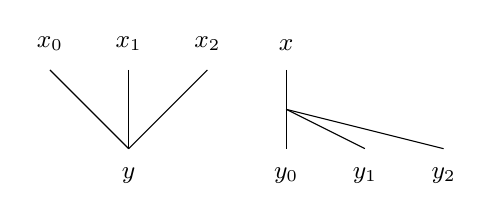
\begin{tikzpicture}
  \node[label={\small $x_0$}] at (-1,1) {};
  \node[label={\small $x_1$}] at (0,1) {};
  \node[label={\small $x_2$}] at (1,1) {};
  \node[label=below:{\small $y$}] at (0,0) {};
  \draw (-1,1) -- (0,0);
  \draw (0,1) -- (0,0);
  \draw (1,1) -- (0,0);

  \node[label={\small $x$}] at (2,1) {};
  \node[label=below:{\small $y_0$}] at (2,0) {};
  \node[label=below:{\small $y_1$}] at (3,0) {};
  \node[label=below:{\small $y_2$}] at (4,0) {};
  \draw (2,1) -- (2,0);
  \draw (2,1/2) -- (3,0);
  \draw (2,1/2) -- (4,0);
\end{tikzpicture}
\\$y=x_0 \dotprod x_1 \dotprod x_2 \quad x=y_0=y_1=y_2$\\

\definition{Circuit Language}
A DSL for describing circuits.\\

\remark{Operations of Circuit Language}
Circuit language has a several operations: \textbf{HIDDEN NOTE IN FILE}.\\
\begin{comment}
\begin{code}
     identity :: Int $\to$ Circuit
e.g. identity 3 = $\begin{tikzpicture}[scale=0.3] \draw (0,0) -- (0,1); \draw (1,0) -- (1,1); \draw (2,0) -- (2,1); \end{tikzpicture}$

     beside :: Circuit $\to$ Circuit $to$ Circuit
e.g. beside ($\begin{tikzpicture}[scale=0.3] \draw (0,0) -- (0,1); \draw (1,0) -- (1,1); \draw (2,0) -- (2,1); \end{tikzpicture}) (\begin{tikzpicture}[scale=0.3] \draw (0,0) -- (0,1); \draw (1,0) -- (1,1); \end{tikzpicture}$) = $\begin{tikzpicture}[scale=0.3] \draw (0,0) -- (0,1); \draw (1,0) -- (1,1); \draw (2,0) -- (2,1); \draw (3,0) -- (3,1); \draw (4,0) -- (4,1); \end{tikzpicture}$
e.g. beside ($\begin{tikzpicture}[scale=0.3] \draw (0,0) -- (0,1); \draw (1,0) -- (1,1); \draw (0,1) -- (1,0); \end{tikzpicture}) (\begin{tikzpicture}[scale=0.3] \draw (0,0) -- (0,1); \draw (1,0) -- (1,1); \draw (2,0) -- (2,1); \draw (1,1) -- (2,0); \end{tikzpicture}$) = $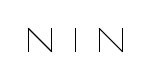
\begin{tikzpicture}[scale=0.3] \draw (0,0) -- (0,1); \draw (1,0) -- (1,1); \draw (2,0) -- (2,1); \draw (3,0) -- (3,1); \draw (4,0) -- (4,1); \draw (0,1) -- (1,0); \draw (3,1) -- (4,0); \end{tikzpicture}$

     above :: Circuit $\to$ Circuit $\to$ Circuit
e.g. above ($\begin{tikzpicture}[scale=0.3] \draw (0,0) -- (0,1); \draw (0,1) -- (1,0); \draw (1,0) -- (1,1); \draw (2,0) -- (2,1); \end{tikzpicture}) (\begin{tikzpicture}[scale=0.3] \draw (0,0) -- (0,1); \draw (1,0) -- (1,1); \draw (1,1) -- (2,0); \draw (2,0) -- (2,1);\end{tikzpicture}$) = $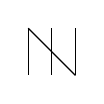
\begin{tikzpicture}[scale=0.3] \draw (0,1) -- (0,-1); \draw (1,1) -- (1,-1); \draw (2,1) -- (2,-1); \draw (0,1) -- (2,-1);\end{tikzpicture}$

     fan:: Int $\to$ Circuit
e.g. fan 4 = $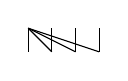
\begin{tikzpicture}[scale=0.3] \draw (0,0) -- (0,1); \draw (1,0) -- (1,1); \draw (2,0) -- (2,1); \draw (3,0) -- (3,1); \draw (0,1) -- (1,0); \draw (0,1) -- (2,0); \draw (0,1) -- (3,0); \end{tikzpicture}$

     stretch :: [Int] $\to$ Circuit $\to$ Circuit
e.g. stretch [1,2,3,2,2] ($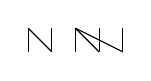
\begin{tikzpicture}[scale=0.3] \draw(0,0) -- (0,1); \draw(1,0) -- (1,1);  \draw(2,0) -- (2,1); \draw(3,0) -- (3,1); \draw(4,0) -- (4,1); \draw(0,1) -- (1,0);  \draw(2,1) -- (3,0);  \draw(2,1) -- (4,0);\end{tikzpicture}$) = ($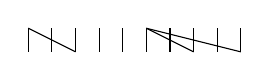
\begin{tikzpicture}[scale=0.3]  \draw(0,0) -- (0,1); \draw(1,0) -- (1,1);  \draw(2,0) -- (2,1); \draw(3,0) -- (3,1); \draw(4,0) -- (4,1); \draw(5,0) -- (5,1); \draw(6,0) -- (6,1); \draw(7,0) -- (7,1); \draw(8,0) -- (8,1); \draw(9,0) -- (9,1); \draw(0,1) -- (2,0);  \draw(5,1) -- (7,0); \draw(5,1) -- (9,0);\end{tikzpicture}$)
e.g. stretch [3,2,4] ($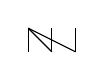
\begin{tikzpicture}[scale=0.3] \draw(0,0) -- (0,1); \draw(1,0) -- (1,1); \draw(2,0) -- (2,1); \draw(0,1) -- (1,0); \draw(0,1) -- (2,0); \end{tikzpicture}$) = ($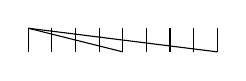
\begin{tikzpicture}[scale=0.3] \draw(0,0) -- (0,1); \draw(1,0) -- (1,1); \draw(2,0) -- (2,1); \draw(3,0) -- (3,1); \draw(4,0) -- (4,1); \draw(5,0) -- (5,1); \draw(6,0) -- (6,1); \draw(7,0) -- (7,1); \draw(8,0) -- (8,1); \draw(0,1) -- (4,0); \draw(0,1) -- (8,0); \end{tikzpicture}$)
\end{code}
\end{comment}
\remark{Operations Descriptions}
$identity\ i$ - Produces a graph with $i$ columns, and no connections.\\
$beside\ c1\ c2$ - Places $c1$ to the right of $c2$ horiztonally next to each other, adds no connections.\\
$above\ c1\ c2$ - Places $c1$ above $c2$, and connects the columns vertically.\\
$fan\ i$ - Produces a graph with $i$ columns and connects the top of the first column to the bottom of the rest.\\
$stretch\ i[]\ c$ - Takes the $j^{th}$ column of $c$ and increases it to $i[j]$ columns. For any columns that were connect, the last column of their new section is connected to the last column of the new section of the target.\\

\example{Deep Embedding of Circuit Language}
The implementation process is:
\begin{enumerate}
  \item Define a datastructure with abstract syntax, maybe recursive.
  \item Define a semantics with an evaluation function.
\end{enumerate}

\textbf{Data Structure}
\begin{code}
data Circuit = Identity Int
             | Beside Circuit Ciruit
             | Above Circuit Ciruit
             | Fan Int
             | Stretch [Int] Ciruit
\end{code}

\textbf{Semantics}\\
The width of a circuit is the number of vertical lines in a circuit.\\
Define a function to find the width of a circuit.
\begin{code}
type Width = Int

width :: Circuit $\to$ Width
width (Identity n)   = n
width (Beside $c_1$ $c_2$)     = width $c_1$ + width $c_2$
width (Above $c_1$ $c_2$)      = width $c_1$
width (Fan n)        = n
width (Stretch ns c) = sum ns
\end{code}

The height of a circuit is the number of layers of a circuit.\\
Define a function to find the height of a circuit.
\begin{code}%TODO move this to own definition
type Height = Int

height :: Circuit $\to$ Height
height (Identity n)   = 1
height (Beside $c_1$ $c_2$)     = 1
height (Above $c_1$ $c_2$)      = height $c_1$ + height $c_2$
height (Fan n)        = 1
height (Stretch ns c) = 1
\end{code}

\textbf{Dependent Semantics}\\
A circuit is well connected if each layer has the same width.\\
A function to check this can be implemented as a dependent semantics, using the $width$ function.
\begin{code}
type Connected = Bool

connected :: Circuit $\to$ Connected
connected (Identity n)   = True
connected (Beside $c_1$ $c_2$)     = connected $c_1$ $\wedge$ connected $c_2$
connected (Above $c_1$ $c_2$)      = connected $c_1$ $\wedge$ connected $c_2$
                         $\wedge$ (width $c_1$ $\equiv$ width $c_2$)
connected (Fan n)        = True
connected (Stretch ns c) = connected c $\wedge$ (width c$\equiv$ length ns)
                         $\wedge$ !(elem 0 ns)
\end{code}

\remark{Extending Deep Embedding}
To extend this deep embedding to include more semantics would be easy, just define more functions.\\
To include new properties in the data type we would need to rewrite all the functions using the data type to work with this new property.\\

\example{Shallow Embedding of Circuit Language}
Implement a semantics to find the width of a circuit.
\begin{code}
type Width   = Int
type Circuit = Width

identity :: Int $\to$ Circuit
identity n = n

beside :: Circuit $\to$ Circuit $\to$ Circuit
beside $c_1$ $c_2$ = $c_1$+$c_2$

above :: Circuit $\to$ Circuit $\to$ Circuit
above $c_1$ $c_2$ = $c_1$

fan :: Int $\to$ Circuit
fan n = n

stretch :: [Int] $\to$ Circuit $\to$ Circuit
stretch ns c = sum ns
\end{code}

\remark{Extending Shallow Embedding}
To extend this shallow embedding to include more semantics would be difficult as we would have to rewrite all the funcitons.\\
However, it would be easy to add new properties to the datastructure as we would just need to implement a new function for this property.\\

\section{The Expression Problem}

\definition{The Expression Problem}
The \textit{expression problem} solves the problem
\begin{quote}
Is it possible to extent the syntax \& semantics of a language in a modular way?
\end{quote}

\definition{Type Constructor} %TODO move this
A function which takes a type and returns a type.%TODO

\definition{Functor}
A functor is a group of data structures which can be mapped over by the same function, $F$.\\
Functors must obey two rules
\begin{enumerate}[label=\roman*)]
  \item Identity, $F\ Identity = Identity$.
  \item Composition, $F(g \dotprod f) = F(g) \dotprod F(f)$.
\end{enumerate}

\definition{fmap}
$fmap$ is the generalised map function for all functors, which all functors implement.\\
The signature of $fmap$ is
\begin{code}
fmap :: (a $\to$ b) $\to$ f a $\to$ f b
\end{code}
f is a type constructor
So $fmap$ takes a function \& a data structure of elements, applies the function to all elements of the data structure and returns the processed datastructure.\\

\remark{Implementations of fmap}
$fmap$ is implemented in different instances of $Functor$.\\
Here is an implementation of $fmap$ of arrays
\begin{code}
instance Functor [] where
  fmap f [ ]  = [ ]
  fmap (x:xs) = (f x) : (fmap f xs)
\end{code}

\definition{Syntatic Sugar List Definition}
The standard definition for lists in Haskell uses syntatic sugar
\begin{code}
data [a] = [ ]
         | $\alpha$ : [a]
\end{code}

\definition{Syntatic-Sugarless List Definition}
this definition uses syntatic sugar. Removing this exposes its generic structure.
\begin{code}
data List a = Empty
            | Cons a (List a)
\end{code}

\definition{Recuresiveless List Definition}
We remove recurrsion from the $List$ datatype \& use $k$ to mark a $k$ontinuation point
\begin{code}
data ListF a k = EmptyF
               | ConsF a k
\end{code}
This is a functor expression.\\

\stepcounter{example} \textbf{Example \arabic{section}.\arabic{example}\ - }\textit{Representing lists as ListFs}
\begin{code}
[5]   $\equiv$ in(ConsF 5 (in EmptyF))
[6,7] $\equiv$ in(ConsF 6 (in (ConsF 7 (in EmptyF))))
\end{code}

\definition{Mutual Recursion}
If two functions or datatypes are defined in terms of each other, they are said to be \textit{mutually recursive}.\\

\definition{Fix}
The datatype $Fix$ provides a fixed point of data. It is defined as
\begin{code}
data Fix f = in (f (Fix f))
\end{code}
where $f$ is a Functor.\\
$Fix$ allows us to generalise all \underline{non-mutually recursive datatypes}.\\
\textit{N.B.} - When considering $Fix$ consider $Maybe$ without a paramter.\\

%TODO define in

\definition{inop}
$inop$ is the opposite of $in$.\\
It is defined as
\begin{code}
inop :: Fix f $\to$ f (Fix f)
inop (in x) = x
\end{code}

\definition{Isomorphic}
Two datastructures, $a$ \& $b$, are isomorphic if there exists two functions, $to$ \& $from$, st
\begin{code}
to   :: a $\to$ b
from :: b $\to$ a

(to . from id) = id
(from . to id) = id
\end{code}

\definition{ListF Functor instance}
A recuresiveless list structure,$ListF$, can be implemented by
\begin{code}
instance Functor (ListF a) where
  fmap :: (x $\to$ y) $\to$ ListF a x $\to$ ListF a y
  fmap f EmptyF      = EmptyF
  fmap f (Consf a x) = Cons a (fx)
\end{code}

\definition{Catamorphism}
Provides a generalisation of Folds.\\
A catamorphism arrises from
\begin{code} %TODO make this better
          fmap cata alg
f(Fix f) --------------> f b
   |  /|\                 |
In |   | inop             | algebra, alg
   |   |                  |
  \|/  |  cata alg       \|/
  Fix f -------------->   b
\end{code}

\definition{Catamorphism Implicit Definition}
By following the arrows of the diagram we can define $cata$.
\begin{code}
    cata :: Functor f $\Rightarrow$ (f b $\to$ b) $\to$ Fix f $\to$ b
    cata alg x = (alg . fmap (cata alg) . inop) x
$\Longleftrightarrow$ cata alg (in x) = alg (fmap (cata alg) x)
\end{code}
\textit{N.B.} - $(f\ b \to b)$ is called the algebra.\\

\proposition{Fix(ListF a) \& List a are isomorphic}
With this being true, we can write $Fix(ListF\ a)$ instead of $List\ a$.
\begin{code}
fromList :: List a $\to$ Fix(ListF a)
fromList Empty       = in (EmptyF)
fromList (Cons x xs) = in(Cons F x (fromList xs))

toList :: Fix(ListF a) $\to$ (List a)
toList = cata alg
  where
    alg :: ListF a (List a) $\to$ List a
    alg EmptyF       = Empty
    alg (ConsF x xs) = Cons x xs
\end{code}
Alternatively
\begin{code}
toList' :: Fix (ListF a) $\to$ [a]
toList' = cata alg
  where
    alg :: ListF a [a] $\to$ [a]
    alg EmptyF       = []
    alg (ConsF x xs) = x : xs
\end{code}
\textit{N.B.} - $k$ has been dropped from $ListF$ declaration as it is provided by $Fix$.\\

\proposition{Implementations of $cata$ - List Length}
Here we define a funciton which returns the length of a $Fix(ListF\ a)$.
\begin{code}
length :: Fix(ListF a) $\to$ Int
length = cata alg
  where
    alg :: ListF a Int $\to$ Int
    alg Empty F     = 0
    alg (ConsF x y) = 1 + y
\end{code}
\textit{N.B.} - $y$ is the length of list calculated so far.

\example{Lazy Evaluation of $length$}
Here we shall perform a lazy evaluation of $length$ of $[7,9]$.
\begin{code}
[7,9] $\equiv$ in(ConsF 7(in (ConsF 9(in EmptyF))))

length(in(ConsF 7(in (ConsF 9(in EmptyF)))))
{length}
cata alg (in (ConsF 7(in (ConsF 9(in EmptyF)))))
{cata}
alg (fmap (cata alg) (ConsF 7(in (ConsF 9 (in (ConsF 9 (in EmptyF)))))))
{fmap}
alg (ConsF 7 (cata alg) (in(ConsF 9 (in EmptyF))))
{alg}
1 + cata alg (in (ConsF 9 (in EmptyF)))
{cata}
1 + alg (fmap (cata alg) (ConsF 9 (in EmptyF)))
{fmap}
1 + alg(ConsF 9 (cata alg) (in EmptyF))
{alg}
1 + 1 + cata alg (in EmptyF)
{cata}
1 + 1 + alg (fmap (cata alg) EmptyF)
{fmap}
1 + 1 + alg EmptyF
{alg}
1 + 1 + 0
{+}
2
\end{code}

\proposition{Implementations of $cata$ - Sum of Integer List}
Here we define a funciton which returns the sum of a $Fix(ListF\ Int)$.
\begin{code}
sum :: Fix (ListF Int) $\to$ Int
sum = cata alg
  where
    alg :: ListF Int Int $\to$ Int
    alg EmptyF      = 0
    alg (ConsF x y) = x + y
\end{code}
\textit{N.B.} - $y$ is the sum so far

\example{Lazy Evaluation of $sum$}
Here we shall perform a lazy evaluation of $sum$ of $[7,9]$.
\begin{code}
[7,9] $\equiv$ in(ConsF 7(in ConsF 9(in EmptyF)))

sum (in(ConsF 7(in (ConsF 9(in EmptyF)))))
{sum}
cata alg (in(ConsF 7(in (ConsF 9(in EmptyF)))))
{cata}
alg (fmap (cata alg) (in(ConsF 7(in (ConsF 9(in EmptyF))))))
{fmap}
alg (ConsF 7 (cata alg) (in (ConsF 9 (in EmptyF))))
{alg}
7 + cata alg (in (ConsF 9 (in EmptyF)))
{cata}
7 + alg (fmap (cata alg) (ConsF 9 (in EmptyF)))
{fmap}
7 + alg(ConsF 9 (cata alg) (in EmptyF))
{alg}
7 + 9 + cata alg (in EmptyF)
{fmap}
7 + 9 + alg (fmap (cata alg) EmptyF)
{alg}
7 + 9 + 0
{+}
16
\end{code}

\subsection{Peano Numbers}

\definition{Peano Number}
A \textit{peano number} is either zero or the successor of another peano number.\\
They have the generic form of
\begin{code}
data Peano = Z          -- zero
           | S Peano    -- successor
\end{code}

\example{Peano number}
The number $3$ can be represented as a peano number by
$$3 = S(S(S\ Z))$$

\proposition{Peano Number Functor}
The functor signature for peano numbers is
\begin{code}
data PeanoF = ZF
            | SF k
\end{code}
The functor instance for peano numbers is
\begin{code}
instance Functor PeanoF where
  fmap :: (a $\to$ b) $\to$ PeanoF a $\to$ PeanoF b
  fmap f ZF     = ZF
  gmap f (SF x) = SF (f x)
\end{code}

\proposition{Implementations of $cata$ - Peano Number to Integer}
This function converts peano numbers to integers
\begin{code}
toInt :: Fix PeanoF $\to$ Int
toInt = cata alg
  where
    alg :: PeanoF Int $\to$ Int
    alg ZF     = 0
    alg (SF x) = 1 + x
\end{code}

\proposition{Implementations of $cata$ - Double Value of Peano Number}
This function doubles the value of a peano number by double the number of $SF$ values.
\begin{code}
double :: Fix PeanoF $\to$ Fix PeanoF
double = cata alg
  where
    alg :: PeanoF $\to$ Fix PeanoF
    alg ZF     = in ZF
    alg (SF x) = in (SF in(SF x))
\end{code}

\subsection{Composing Languages}

\definition{Coproduct of Functors}
The \textit{coproduct of functors} is defined as
\begin{code}
data (f :+: g) a = L (f a)
                 | R (g a)
\end{code}
So given two functors $f$ \& $g$, it produces a functor $(f :+: g)$ which executes a different function depending on the type of the input $a$.\\
The functor instance is
\begin{code}
instance (Functor f, Functor g) => Functor (f :+: g) where
  fmap :: (a $\to$ b) $\to$ (f :+: g) a $\to$ (f :+: g) b
  fmap f (L x) = L (fmap f x)
  fmap f (R y) = R (fmap f y)
\end{code}
\textit{N.B.} - $x :: f\ a\ \&\ y :: g\ a$.

\definition{Junction of Algebras}
To reduce a $Fix$ expression on a \textit{coproduct of functors} to simple $a \to b$ we use a \textit{junction of algebras}. Defined as
\begin{code}
($\nabla$) :: (f a $\to$ a) $\to$ (g a $\to$ a) $\to$ (f :+: g)a $\to$ a
(flag $\nabla$ galg)(L x) = falg x
(flag $\nabla$ galg)(R x) = galg x
\end{code}

\example{Coproduct of Functors}
We previously defined a language for addition.
\begin{code}
data Expr = Val Int
          | Add Expr Expr
\end{code}
Which can be expressed without recursion as
\begin{code}
data ExprF = ValF Int
           | AddF k k
\end{code}
So $Fix\ ExprF=Expr$.\\
A functor signature for multiplication is
\begin{code}
MulF' :: k $\to$ k $\to$ MulF k
MulF k = MulF' k k
\end{code}
This can be instanced with
\begin{code}
instance Functor MulF where
  fmap f (MulF x y) = Mul (f x) (f y)
\end{code}
By defining the algebras
\begin{code}
add : ExprF Int $\to$ Int
add (ValF x) = x
add (AddF x y) = x + y

mul:: MulF Int $\to$ Int
mul (MulF x y) = x * y
\end{code}
We can use the coproduct of functors to create a single evaluation for both addition \& multiplicaiton.
\begin{code}
eval :: Fix (ExprF :+: MulF) $\to$ Int
eval = cata (add $\nabla$ mul)
\end{code}

\section{Parsers}

\subsection{Backus-Naur Form}

\definition{Backus-Naur Form, BNF}
\textit{Backus-Naur Form} is a language used to express the shape of grammar.\\
It was invented in 1958 for express of Algol.\\

\remark{Syntax of Backus-Naur Form}
A \textit{Backus-Naur Form} statment is made up of
\begin{itemize}
  \item[-]$\varepsilon$, empty string.
  \item[-]$<a>$, non-terminal.
  \item[-]$``a"$, terminal.
  \item[-] $a|b$, choice between $a$ or $b$.
\end{itemize}

\remark{Additional Syntax of Backus-Naur Form}
\textit{Backus-Naur Form} is usually extended to include the following, although they can be achieved using the previous features.
\begin{itemize}
  \item[-] $[a]$, optional $a$.
  \item[-] $(a)$, grouping $a$.
  \item[-] $a*$, $\geq0$ repitions $a$.
  \item[-] $a+$, $\geq1$ repitions $a$.
\end{itemize}

\example{Expressing Numbers in BNF}
The following represents a single digit
\begin{code}
<digit> ::= "0" | "1" | "2" | "3" | "4" | "5" | "6" | "7" | "8" | "9"
\end{code}
This cna be used to approximate numbers
\begin{code}
<num> ::= <digit>
        | <digit> <num>
\end{code}

\example{Expressing Addition in BNF}
In haskell we define addition as
\begin{code}
data Expr = Val Num
          | Add Num Expr
\end{code}
In BNF it can be expressed as
\begin{code}
<expr> ::= <num>
         | <num> "+" <expr>
\end{code}

\remark{Ambiguous Grammars}
Some grammar definition are not precise enough, as they can be interpreted in multiple ways.\\

\example{Ambiguous Grammars}
Consider the following definition for addtion, in BNF
\begin{code}
<expr> ::= <num>
         | <expr> "+" <expr>
\end{code}
This is ambiguous as, should it be given $1+2+3$ it doesn't define whether to evaluate it as $(1+2)+3$ or $1+(2+3)$.\\
\textit{N.B.} - The issue with this definition occurs in \textit{recursive-descent parses}. %TODO define recursive-descent parses

\subsection{Paull's Modified Algorithm}

\definition{Paull's Modified Algorithm}
\textit{Paull's Modified Algorithm} is used to remove recursion from grammar definitions.\\ %TODO check\extend this
Given
\begin{code}
A ::= A$\alpha_1$ | $\dots$ | A$\alpha_n$ | $\beta_1$ | $\dots$ | $\beta_m$
\end{code}
where $A$ is a non-terminal and $\alpha_i, \beta_j$ are \textit{BNF} expressions.\\
Applying \textit{Paull's Modified Algorithm} refactors this to
\begin{code}
A  ::= $\beta_1$A' | $\dots$ | $\beta_m$A'
A' ::= $\alpha_1$A' | $\dots$ | $\alpha_n$A'| $\varepsilon$
\end{code}

\example{Paull's Modified Algorithm}
Given the expression
\begin{code}
<expr> ::= <num>
         | <expr> "+" <expr>
\end{code}
this is refactored to
\begin{code}
<expr>  ::= <num> <expr'>
<expr'> ::= "+" <expr> <expr'> | $\varepsilon$
\end{code}

\subsection{Parsers}

\definition{Parser}
A parser is a funciton that takes in a list of characters (string) \& returns an item that has been parsed, along with the unconsumed string.\\
The haskell data type for this is
\begin{code}
newtype Parses a = Parse (String $\to$ [(a, String)])
\end{code}

\proposition{Parse}
We can use a parser by defining the function \textit{parse}.
\begin{code}
parse :: Parser a $\to$ String $\to$ [(a, String)]
parse (Parser px) s = px s
\end{code}

\proposition{Fail Parser}
This parser always returns an empty list, showing the parse has failed.
\begin{code}
fail :: Parser a
fail = Parser ($\lambda$ ts $\to$ [])
\end{code}
When implemented we get
\begin{code}
parse fail "Hello" = [ ]
\end{code}

\proposition{Item Parser}
This parser returns a single character when passed a string.
\begin{code}
item :: Parser Char
item = Parser ($\lambda$ ts $\to$ case ts of
                [] $\to$ []
                (t:ts') $\to$ [(t,ts')]
              )
\end{code}
When implemented we get
\begin{code}
parse item "Hello" = [('H', "ello")]
\end{code}

\proposition{Look Parser}
This parser is used to look at the input stream without consuming anything.
\begin{code}
look :: Parser String
look = Parser ($\lambda$ ts $\to$ [(ts, ts)])
\end{code}
When implemented we get
\begin{code}
parse look "Hello" = [("Hello", "Hello")]
\end{code}

\remark{Transforming Parsers}
Sometimes we want to transform our parses so they produce values of a different type.\\
this is achieved by given a functor instance for parses.
\begin{code}
instance Functor Parser where
  fmap f (Parser ps) = Parser ($\lambda$ ts $\to$ [(f x, ts') | (x,ts') $\leftarrow$ ts])
\end{code}
This can be visualised as\\
\begin{tabular}{|ccccc|}
\hline
&&ts&&\\
\hline
x&\vline&ts'&&\\
\hline
f x&\vline&ts'&&\\
\hline
\end{tabular}\\
%TODO we can use this to define a parse for

\definition{Combinations}
Combinations are used to combine parsers, they have different definitions which can be utilised for a desired effect.
\begin{code}
(<$\mathdollar$>) :: (a $\to$ b) $\to$ Parser a $\to$ Parser b
f <$\mathdollar$> px = fmap f px
\end{code}
There are variations on this, such as
\begin{code}
(<$\mathdollar$) :: a $\to$ Parser b $\to$ Parser a
x <$\mathdollar$ py = fmap (cost x) py
\end{code}

\remark{Space is a Combinator}
Consider $f\ x$, the space between $f$ and $x$ can be considered as an operation which takes $f$ \& $x$ as inputs and then applies $f$ to $x$.\\

\proposition{Skip Parse}
This function parses an input but outputs nothing useful.
\begin{code}
skip :: Parser a $\to$ Parse ()
skip px = () <$\mathdollar$ px
\end{code}

\definition{Applicative Class}
This class defines the functions $pure$ and $(<*>)$.
\begin{code}
class Functor f => Applicative f where
  pure  :: a $\to$ f a
  (<*>) :: f (a $\to$ b) $\to$ fa $\to$ fb
\end{code}

\proposition{Parser Applicative Class Instance}
The Applicative class can be instanced for Parsers as
\begin{code}
instance Applicative Parser
  where
    pure x = Parse ($\lambda$ ts $\to$ [(x,ts)])
    (Parser pf) <*> (Parse px) = Parser ($\lambda$ ts $\to$
                                        [ (f x, ts'')
                                        | (f,ts') $\leftarrow$pf ts
                                        , (x,ts'')$\leftarrow$px ts'])
\end{code}
The defined operation first parses a function, then a value and then applies the function to this value.\\

\proposition{Variations of ap operator}
\textit{Inverse Ap}\\
Say we wanted to parse a value, then parse a function and then apply the function to the value we use the following.\\
\begin{code}
(<**>) :: Parser a$\to$Parser (a$\to$b)$\to$Parser b
(Parser px) <**> (Parser pf) = Parse ($\lambda$ ts$\to$
                                     [ (f x, ts'')
                                     | (x,ts') $\leftarrow$px ts
                                     , (f,ts'')$\leftarrow$pf ts'])
\end{code}
\textit{Left ap}\\
If we want to only use the Parser to the left of the operator we use the following.\\
\begin{code}
(<*) Parser a$\to$Parse b$\to$Parse a
\end{code}
\textit{Right ap}\\
If we want to only use the Parser to the right of the operator we use the following.\\
\begin{code}
(*>) Parser a$\to$Parse b$\to$Parse b
\end{code}

\remark{Implementation of Applicative Parser}
When applied we get $parse (pure\ 5) ``Hello" = [(5,``Hello")]$.\\

\proposition{Apply Function of Parse Output}
Consider a parse which results in\\
\begin{tabular}{|lllll|}
\hline
&&ts&&\\
\hline
(a$\to$b$\to$x)\vline&x::a\vline&y::b\vline&z::c\vline&ts'\\
\hline
\end{tabular}\\
We want to apply a function to the different outputs of hte parse. To make this function which does this we can use $<*>$ as
\begin{code}
f <*> px <*> py <*> pz
\end{code}
\textit{N.B.} - The $f$ here is given to us \& we didn't need to parse it.\\

\definition{Monoidal Type Class}
The Monoidal type class is equivalent ot Applicative.
\begin{code}
class Monoidal f
  where
    unit :: f ()
    mult :: f a$\to$f b$\to$f (a,b)
\end{code}

\proposition{Parser Monoidal Class Instance}
The parser datatype can be instanced for monoidal class by
\begin{code}
instance Monoidal Parser
  where
    unit                         = Parser ($\lambda$ ts $\to$ [((), ts)])
    mult (Parser px) (Parser py) = Parser ($\lambda$ ts $\to$ [ ((x,y),ts'')
                                          | (x,ts')  $\leftarrow$ px ts
                                          | (t,ts'') $\leftarrow$ py ts'])
\end{code}
Here the $x$ is parsed first and then $y$ is parsed from the string remaining from that.\\

\remark{mult as a Binary Operator}
It is useful to make $mult$ a binary operator
\begin{code}
(<$\sim$>) :: Monoidal f$Rightarrow$f a$\to$f b$\to$f (a,b)
px <$\sim$> py = mult px py
\end{code}

\remark{Variations of mult Binary Operator}
We can derive left and right variables of $<~>$.
\begin{code}
(<$\sim$) :: Monoidal f$\Rightarrow$f a$\to$f b$\to$f a
px <$\sim$ py = fst <$\mathdollar$> (px <$\sim$> py)

($\sim$>) :: Monoidal f$\Rightarrow$f a$\to$f b$\to$f b
px $\sim$> py = snd <$\mathdollar$> (px <$\sim$> py)
\end{code}

\subsection{Alternatives}

\definition{Alternative Type Class}
We can produce parsers that can deal with choices in a grammar
\begin{code}
class Alternative f
  where
    empty :: f a
    (<|>) :: f a$\to$f a$\to$f a
\end{code}

\remark{Parser Alternative Class Instance}
The Parse dataype can be instanced for the Monoindal class by
\begin{code}
instance Alternative Parser
  where
    empty = fail
    (Parser px) <|> (Parser py) = Parser ($\lambda$ ts$\to$px ts++py ts)
\end{code}

\remark{Equivalents to $<|>$}
\begin{code}
parse (px <|> py) ts = (parse px ts) ++ (parse py ts)
\end{code}

\definition{choice}
$choice$ is used to extend $<|>$ to accept many input parsers.
\begin{code}
choice :: [Parser a] $\to$ Parser a
choice pxs = foldr (<|>) pxs
\end{code}

\definition{Combinator - $<:>$}
We can define a combinator that appends the result of a parse into others
\begin{code}
(<:>) :: Parser a $\to$ Parser [a] $\to$ Parser [a]
px <:> pxs = (:) <$\mathdollar$> px <*> pxs
\end{code}
\textit{N.B.} - $(:)\ <\mathdollar>\ px\ <*>\ pxs = \left((:)\ <\mathdollar>\ px\right)\ <*>\ pxs$.\\

\proposition{Backus-Naur Form Parsers}
We can define combinators that correspond to $'+'$ \& $'*'$ from Backus-Naur Form.
\begin{enumerate}[label=\roman*)]
  \item $e+$ is written $some\ e$.
  \item $e*$ is written $many\ e$.
\end{enumerate}
\begin{code}
some :: Parser a $\to$ Parser [a]
some px = px <:> many px
many :: Parser a $\to$ Parser [a]
many px = some px <|> pure
\end{code}
$some$ parses one $px$ and adds it to the result of $many\ px$.\\
$many\ px$ returns $some\ px$, if this does not exist then returns $empty$.

\subsection{Monadic Parsing}

\remark{Motivation}
Sometimes we want to control the flow of a $Parser$ to depend on what was parsed.\\
Suppose we have $px::Parser\ a$ we can define a function $f::a\to Parser\ b$.\\
The function $f$ inspects the value $x$ which came from $px$ and produces a new Parser accordingly.\\
the result should be a parser of type $Parser\ b$.\\

\definition{Monadic Instance of Parser}
\begin{code}
instance Monad Parser where
-- return :: a $\to$ Parser a
   return = pure        -- From Applicative
-- (>>=) :: Parser a $\to$ (a$\to$Parser b) $\to$ Parser b
   (Parser px) >>= f = Parser ($\lambda$ ts $to$
                              concat [parse (fx) ts'
                                     | (x,ts')$\leftarrow$px ts])
\end{code}

\proposition{Implementing Monadic Combinator}
To use the monadic combinator we combina  parser with a function.\\
The $satisfy$ parser takes a function that is a predicate of $Chars$ and returns the parse value if it satisfies the predicate.
\begin{code}
satisfy :: (Char$\to$Bool)$\to$Parser Char
satisfy p = item >>= ($\lambda$ t $\to$ if p t
                             then pure t
                             else empty)
\end{code}

\proposition{satisfy Without Monadic Definition}
$satisfy$ can be defined without using the monadic definition.
\begin{code}
satisfy :: (Char$\to$Bool)$\to$Parser Char
satisfy p = Parser ($\lambda$ ts $to$ case ts of
                    []$\to$empty
                    (t:ts')$\to$[(t,ts')|p t])
\end{code}

\definition{Char Parser}
We can parse a single character as follows
\begin{code}
char :: Char$\to$Parser Char
char c = satisfy (c==)
OR
char c = satisft ($\lambda$ c'$\to$c'==c)
\end{code}
\textit{N.B.} - $parse\ (char\ 'x') ''xys" = [('x',"yz")]$.\\

\subsection{Long Example}
Consider begining given the following definitions:
\begin{code}
expr = term | expr ``+" term
term = fact | term ``*" fact
fact = numb | ``(" expr ``)"
numb = ``0" | ``1" | $\dots$ | ``9"
\end{code}
These definitions are left recurvise which is bad as the compiler can end up in a loop.\\
We can change this by using Paull's Algorithm.
\begin{code}
expr = term expr'
expr' = ``+" term expr' | $\varepsilon$

term = fact term'
term' = ``*" fact term' | $\varepsilon$
\end{code}
From these we can make corresponding datatypes.\\
Each non-terminals becomes a datatpe, whereas the alternations are constructors.
\begin{code}
data Expr  = ExprTerm Term Expr'
data Expr' = Expr'Add Term Expr' | ExprEps'

data Term  = TermFact Fact Term'
data Term' = Term'Mul Fact Term' | TermEps'

data Fact = FactNumb Int | FactPar Expr
\end{code}
Now we have usable datastructure we can make a Parser.\\
These correspond to Paull's Definition.
\begin{code}
expr :: Parser Expr
expr = Expr <$\mathdollar$> term <*> expr

expr' :: Parse Expr'
expr' = Expr'Add <$\mathdollar$ char '+' <*> term <*> expr'
    <|> Expr'Eps <$\mathdollar$ pure()

term :: Parser Term
term = TermFact <$\mathdollar$> fact <*> term'

term' :: Parser Term'
term' = Term'Mul <$\mathdollar$ char '*' <*> fact <*> term'
    <|> Term'Eps <$\mathdollar$ pure ()

fact = FactNumb <$\mathdollar$> numb
   <|> FactPar <$\mathdollar$ char '(' <*> expr <* char ')'

numb :: Parse Int
numb = read <$\mathdollar$> digits

digit :: Parser Char
digit = satisfy isDigit

digits :: Parser Int
digits = cull (some digit)
\end{code}
These can be applied to produce the following results
\begin{code}
parse (numb) ``12hh3124" = [(12, ``hh3124")]
\end{code}

%TODO define read & cull
\remark{Debugging}
By enabling $derive\ Show$ on all the previous structures will print when to terminal when required, making debuggin easier.\\

\remark{When to use $<>$, $<$ or $>$}
Often it is best to write out the expression in full and then remove parentenses are required.

\subsection{Chain for Left-Recursions}

\remark{Motivation}
The problem with ambiguous grammars, which are left recursive, can be solved with \textit{Paull's Algorithm}.
\begin{code}
<expr> ::= <number>
         | <expr> "+" <expr>
\end{code}
However, without applying \textit{Paull's Algorithm} we have a nice datatype
\begin{code}
data Expr = Num Int
          | Add Expr Expr
\end{code}

\definition{$chainl_1$}
$chainl_1$ is used to parse from the original grammar into this datastructure, assuming the operation ("+") is left associative.\\
It's signature is
\begin{code}
chainl$_1$ :: Parser a$\to$Parser (a$\to$a$\to$a)$\to$Parser a
\end{code}
\textit{N.B.} - $chainr_1$ is used when the operation is right associative.\\

\example{$chainl_1$}
Consider making a parser for the following datatype
\begin{code}
data Expr = Num Int
          | Add Expr Expr
\end{code}
$chainl_1$ can be used to achieve this
\begin{code}
expr :: Parser Expr
expr = chainl$_1$ number add
\end{code}
This can be expanded to create a parser for addition
\begin{code}
add :: Parser (Expr$\to$Expr$\to$Expr)
add = Add <$\mathdollar$ tok "+"
\end{code}

\section{The Free Monad}
\textit{AKA Generic Syntax or Abstract Syntax Trees}.\\

\proposition{Abstract Syntax Tree}
When analysing the syntax of a language, we first want to establish which symbols are operations and which are variables.\\
We can use a tree to show the relationships between variables and operations.\\
The elements in diamonds are operations \& those in rectangles are variables.\\

\remark{Compiler}
Opteration symbols tell the compiler to add command to stack.\\
Variable symbols tell the compiler to load the value into memory and add to stack.\\

\example{Abstract Syntax Trees}
Suppose we are interested in giving a semantics to a language for addition.\\
The syntax could look like
$$(x+y)+z$$
Here we are not considering whether $x,\ y$ \& $z$ are numbers yet.\\
This example can be consider as the syntax tree\\
\begin{tikzpicture} [node distance = 2cm, auto]
  \node[op] {"+"}
    child {node[op] {"+"}
      child {node[var] {x}}
      child {node[var] {y}}
    }
    child {node[var] {z}};
\end{tikzpicture}\\

\remark{Interpreting Free Monad Trees}
We interpret free monad trees in two stages:
\begin{enumerate}[label=\roman*)]
  \item Generator - Change variables into values;
  \item Algebra - Evaluate the operations using these values.
\end{enumerate}
A visualised example of this is\\
\begin{tikzpicture} [node distance = 2cm, auto]
  \node[op] {+}
    child {node[var] {x}}
    child {node[var] {y}};
\end{tikzpicture}
$\xrightarrow{Generator}$
\begin{tikzpicture} [node distance = 2cm, auto]
  \node[op] {+}
    child {node {3}}
    child {node {7}};
\end{tikzpicture}
$\xrightarrow{Algebra}$
\begin{tikzpicture} [node distance = 2cm, auto]
\node {+}
  child {node {3}}
  child {node {7}};
\end{tikzpicture}\\

\definition{Free Monad}
The free monad $Free\ f\ a$ provides syntax trees whose nodes are shaped by \textit{functor} $f$ and whose variables come from the type $a$.\\
It is defined as
\begin{code}
data Free f a = Var a
              | Op (f (Free f a))
\end{code}
\textit{N.B.} - The $Op$ constructor is similar to the definition for $Fix$.\\

\proposition{Functor Instance of Free Monad}
Consider $(Op\ op)::Free\ f\ a$, here $op::f(Free\ f\ a)$.\\
Using $fmap$ we want to make it of type $f(Free\ f\ b)$.\\
This can be done using $fmap(fmap\ f)$ since $fmap::f(Free\ f\ a)\to f(Free\ f\ b)$ which will evaluate the outside of $op$ and $(fmap\ f)::Free\ f\ a\to Free\ f\ b$ which will evaluate the inside of $op$.
\begin{code}
instance Functor f $\Rightarrow$ Functor (Free f)
  where
    -- fmap :: (a$\to$b)$\to$(Free f a)$\to$(Free f b)
       fmap f (Var x) = Var (f x)
       fmap f (Op op) = Op (fmap (fmap f) op)
\end{code}

\example{Free Monad - Addition}
Consider the double addition example.\\
We can define the \textit{shape} of $+$
\begin{code}
   data AddF k = AddF k k
OR data AddF k = k :+ k
\end{code}
\textit{N.B.} - The tree for double addition can be expressed with the following values of type $Free\ AddF\ String$ and $Op\ (AddF\ (Op\ (AddF\ (Var\ ``x") (Var\ ``y"))) (Var\ ``z"))$.\\

\definition{extract}
The second stage extracts semantics by applying an algebra.\\
This is done by a recursive function defined as
\begin{code}
extract :: Functor f$\Rightarrow$(f b$\to$b)$\to$Free f b$\to$b
extract alg (Var x) = x
extract alg (Op op) = alg (fmap (extract alg) op)
\end{code}
\textit{N.B.} - The second clause here is identical to $cata$.\\

\definition{eval}
By combining the generator \& algebra stage we can produce an evaluation function
\begin{code}
eval :: Functor f$\Rightarrow$(f b$\to$b)$\to$(a$\to$b)$\to$Free f a$\to$b
eval alg gen = extract alg $\circ$ fmap gen
\end{code}
\textit{N.B.} - $fmap\ gen$ executes the first stage \& $extract\ alg$ excutes the second.\\

\example{Addition Language}
Consider the $AddF$ functor from earlier.\\
First we define an algebra for the functor
\begin{code}
alg :: AddF Int$\to$Int
alg (x :+ y) = x + y
\end{code}
Now we define a generator from the type of our variables to integers.
\begin{code}
type Var = String
env :: Var$\to$Int
env "x" = 3
env "y" = 5
env _   = 0
\end{code}
Here is a visualised example of the evaluation process\\
\begin{tikzpicture} [node distance = 2cm, auto]
  \node[op] {:+}
    child {node[op] {:+}
      child {node[var] {x}}
      child {node[var] {y}}
    }
    child {node[var] {z}};
\end{tikzpicture}
$\xrightarrow{fmap\ env}$
\begin{tikzpicture} [node distance = 2cm, auto]
  \node[op] {:+}
    child {node[op] {:+}
      child {node {3}}
      child {node {5}}
    }
    child {node {0}};
\end{tikzpicture}
$\xrightarrow{extract\ add}$
\begin{tikzpicture} [node distance = 2cm, auto]
  \node {+}
    child {node {+}
      child {node {3}}
      child {node {5}}
    }
    child {node {0}};
\end{tikzpicture}\\
\textit{N.B.} - This is the evaluation of $eval\ add\ env$.\\

\example{Variable Collector}
In this example we will collect all the variables in an expression as a list.\\
So $``x+y+z"\to[``x",``y",``z"]$.\\
We define a function for this as
\begin{code}
vars :: Free AddF Var$\to$[Var]
vars = eval alg gen
  where
    -- gen :: Var$\to$[Var]
    -- alg :: AddF [Var]$\to$[Var]
       gen x          = [x]
       alg (xs :+ ys) = xs ++ ys
\end{code}
Here is a visualised example of the evaluation process\\
\begin{tikzpicture} [node distance = 2cm, auto]
  \node[op] {:+}
    child {node[op] {:+}
      child {node[var] {x}}
      child {node[var] {y}}
    }
    child {node[var] {z}};
\end{tikzpicture}
$\xrightarrow{extract\ gen}$
\begin{tikzpicture} [node distance = 2cm, auto]
  \node[op] {:+}
    child {node[op] {:+}
      child {node {["x"]}}
      child {node {["y"]}}
    }
    child {node {["z"]}};
\end{tikzpicture}
$\xrightarrow{fmap\ alg}$
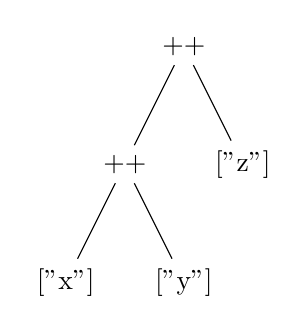
\begin{tikzpicture} [node distance = 2cm, auto]
  \node {++}
    child {node {++}
      child {node {["x"]}}
      child {node {["y"]}}
    }
    child {node {["z"]}};
\end{tikzpicture}

\proposition{Division Operation}
Suppose we want to add an new operation to our arithmetic language that performs division.\\
We can do this with the following datatype
\begin{code}
data DivF k = DivF k k
\end{code}
If we want to provide a semantics that collects all the variables we must provide an algebra as follow
\begin{code}
divVars::DivF[Var]$\to$[Var]
divVars (DivF xs ys)=xs++ys
\end{code}
If we only want to work with division we can use the following
\begin{code}
evalDiv::Free DivF Var$\to$[Var]
evalDiv=eval alg gen
  where
    gen::Var$\to$[Var]
    gen x=[x]
    alg::DivF[Var]$\to$[Var]
    alg (DivF xs ys)=xs++ys
\end{code}
If we want a language with both addition and division we need to take the co-product of \textit{AddF} and \textit{DivF}
\begin{code}
vars::Free (AddF:+:DivF)Var$\to$[Var]
vars=eval alg gen
  where
    gen x=[x]
    alg::(AddF:+:DivF)[Var]$\to$[Var]
    alg (L(AddF xs ys))=xs++ys
    alg (R(DivF xs ys))=xs++ys
\end{code}
When performing division we cannot simply do $\frac{x}{y}$ incase $y=0$.\\
Then we use the \textit{Maybe} datatype
\begin{code}
expr::Free(AddF:+:DivF)Var$\to$Maybe Double
expr=eval alg gen
  where
    gen=env$^[1]$
    alg(L(AddF x y))=mAdd x y
    alg(R(DivF x y))=mDiv x y

    mAdd::Maybe Double$\to$Maybe Double$\to$Maybe Double
    mAdd (Just x) (Just y)= Just(x+y)
    mAdd _         _      = Nothing

    mDiv::Maybe Double$\to$Maybe Double$\to$Maybe Double
    mDiv _        (Just 0) = Nothing
    mDiv (Just x) (Just y) = Just (x/y)
    mDiv _        _        = Nothing
\end{code}

\subsection{Failure}

\definition{Fail Datatype}
We need a syntax for failure
\begin{code}
data Fail k = Fail
\end{code}

\proposition{Functor instance of Fail}
The functor instance of \textit{Fail} shows us that computations cannot follow a fail.
\begin{code}
instance Functor Fail
  where
    fmap f Fail=Fail
\end{code}

\proposition{Fail and Division}
Here we integrate \textit{Fail} with the division operation defined in \textbf{Section \arabic{section}.\addtocounter{subsection}{-1}\arabic{subsection}\addtocounter{subsection}{1}}.
\begin{code}
evalFail::Free DivF Double$\to$Free Fail Double
evalFail=eval alg gen
  where
    gen::Double$\to$Free Fail Double
    gen x=Var x
    alg::DivF (Free Fail Double)$\to$Free Fail Double
    alg (DivF (Var x) (Var 0))=Op Fail
    alg (DivF (Var x) (Var y))=Var (x/y)
    alg _                     =Op Fail
\end{code}
This process converts a tree to another tree, checking for possible failures.\\

\subsection{Substitution}

\remark{Motivation}
Consider \textit{'x+7'}.\\
We can evaluate this into a new syntax tree where we have a notion of substitution, where we might bind \textit{'x'} to another expression rather than a constant $x\mapsto4+5$.\\
Then we expect $x+7\mapsto(4+5)+7$.\\

\proposition{Tree Representation}
The initial epxression and substitution in \textbf{Remark \arabic{section}.\arabic{remark}} can be represented by the following trees
\begin{tikzpicture} [node distance = 2cm, auto]
  \node[op] {+}
    child {node[var] {x}}
    child {node[op]  {7}};
\end{tikzpicture}
$x\mapsto$
\begin{tikzpicture} [node distance = 2cm, auto]
  \node[op] {+}
    child {node[var] {4}}
    child {node[op]  {5}};
\end{tikzpicture}\\
\textit{N.B.} - Here we consider \textit{'4'}, \textit{'5'} \& \textit{'7'} to be operations.\\

\remark{Notation}
Consider an expression $e$ with a variable $x$, where $x$ is substituted by $e'$.\\
We denoted this by
$$e[x\mapsto e']$$
Occasionaly $e[x\backslash e']$ or $e[e'/x]$ are used.\\

\definition{$(>>=)$}
Substitution is defied by $(>>=)$
\begin{code}
(>>=)::Free f a$\to$(a$\to$Free f b)$\to$Free f b
Var x  >>= f=f x
Op  op >>= f=Op(fmap (>>= f) op)
\end{code}
This applies the substitution, $(>>=) f$, to all lower layers of the tree.

\subsection{Non-Determinism}

\definition{Non-Deterministic Computation}
A \textit{Non-Deterministic Computation} is a computation that provides the choice between two different computations.\\
Consider $p\square q$ is the program that fives answers $p$ or $q$\\
\begin{tikzpicture} [node distance = 1cm, auto]
  \node[op] {Or}
    child {node[var] {p}}
    child {node[var] {q}};
\end{tikzpicture}

\remark{Square Root}
The square root is a non-deterministic computation as it produces a pair or results, one positive \& one negative.\\

\example{Non-Deterministic Computation}
Suppose a computation produces the possible results $3$,$4$ or $6$.\\
We want to return a list containing these results.\\
The evalutation function can be visualised as\\
\begin{tikzpicture} [node distance = 1cm, auto]
  \node[op] {Or}
    child {node[op] {Or}
      child {node[var] {3}}
      child {node[var] {4}}
    }
    child {node[var] {6}};
\end{tikzpicture}
$\xrightarrow{gen}$
\begin{tikzpicture} [node distance = 1cm, auto]
  \node[op] {Or}
    child {node[op] {Or}
      child {node {[3]}}
      child {node {[4]}}
    }
    child {node {[6]}};
\end{tikzpicture}
$\xrightarrow{alg}$
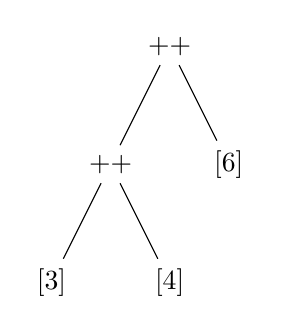
\begin{tikzpicture} [node distance = 1cm, auto]
  \node {++}
    child {node {++}
      child {node {[3]}}
      child {node {[4]}}
    }
    child {node {[6]}};
\end{tikzpicture}

\proposition{Implementation}
We can expression non-determinism by the syntax
\begin{code}
data Or k=Or k k
\end{code}
We need this ot be a function in order to use the evaluator
\begin{code}
instance Functor Or
  where
    fmap f (Or x y)=Or (f x) (f y)
\end{code}
Now we can dfine an evaluation function
\begin{code}
list::Free Or a$to$[a]
list=eval alg gen
  where
    gen::a$to$[a]
    gen x=[x]
    alg::Or [a]$to$[a]
    alg (Or xs ys)=xs++ys
\end{code}
Another interpretation of these trees is to simply returh the first result.\\
This can be done by the following code
\begin{code}
once :: Free Or a$to$Maybe a
once = eval alg gen
  where
    gen::a$to$Maybe a
    gen x=Just x
    alg::Or(Maybe a)$to$Maybe a
    alg (Or Nothing  y)=y
    alg (Or (Just x) y)=Just x
\end{code}

\definition{Non-Determinism Syntax}
The above approach works but we want to signal if there is no solution.\\
We do this using Nondeterminism, which can be given by the following syntax
\begin{code}
type Nondet a=(Fail:+:Or) a
\end{code}

\remark{Nondet Trees}
Trees of type \textit{Free\ (Nondet)\ a} have shape\\
\begin{tikzpicture} [node distance = 1cm, auto]
  \node[op] {Or}
    child {node[op] {Fail}}
    child {node[op] {Or}
      child {node[var] {3}}
      child {node[op] {Fail}}
    };
\end{tikzpicture}

\definition{Semantics for Nondet Languages}
We give semantics to nondet languages by providing a generator and an algebra.\\
\begin{code}
list::Free Nondet a$to$[a]
list = eval alg gen
  where
    gen::a$to$[a]
    gen x=[x]
    alg::Nondet [a]$to$[a]
    alg (L Fail)=[]
    alg (R (Or x y))=x++y
\end{code}
\textit{N.B.} - The semantics for \textit{once} is similar.\\

\subsection{Alteration}

\remark{Motivation}
A different approach, than the \textit{Or}, is to model a pair of \textit{k} values as a function from \textit{Bool}.\\

\definition{Alternative Datatype}
We can define a data type for this as
\begin{code}
data Alt k=Alt (Bool$\to$k)
\end{code}
We pass \textit{True} when we want the first child and \textit{False} for the second.\\

\definition{Alt Functor Definition}
The \textit{Functor} instance for \textit{Alt}
\begin{code}
instance Functor Alt
  where
    fmap f (Alt k)=Alt (f.k)
\end{code}

\definition{Non-Determinism Datatype}
We can give alternative semantics for non-determinism using \textit{Alt}
\begin{code}
type Nondet' a=(Fail :+: Alt) a
\end{code}

\definition{list}
We can redefine \textit{list} using the new \textit{Nondet'} definition
\begin{code}
list::Free Nondet' a$\to$[a]
lsit=eval alg gen
  where
    gen::a$\to$[a]
    gen x=[x]
    alg::Nondet'[a]$\to$[a]
    alg (L Fail)   =[]
    alg (R (Alt k))=(k True)++(k False)
\end{code}
\textit{N.B.} - This shows that the parameter to a syntax function sometimes has the form of a function.\\

\subsection{State}

\definition{Stable Computation}
A stable computation can be modelled by having two operations \textit{GET} \& \textit{Put}.\\
These can be defined as
\begin{code}
data State s k=Put s k
              |Get (s$\to$k)
\end{code}

\remark{}
The intutition of \textit{State} is that \textit{Put s k} will put the value \textit{s} into the state, before continuing with the computation in \textit{k}.\\
The \textit{Get h} operation will only continue when \textit{h::s$\to$k} is given a variable of type \textit{s}.\\

\proposition{Sematic Domain of State}
The semantic domain for \textit{State} is a function of type
\begin{code}
s$\to$(a,s)
\end{code}
The first \textit{s} is the old state \& the second is the new state.\\
This is a carrier for stateful computations.\\

\definition{evalState}
\begin{code}
evalState::Free (State s) a$\to$(s$\to$(a,s))
evalState=eval alg gen
  where
    gen::a$\to$(s$\to$(a,s))
    gen x=$\lambda$s$\to$(x,s)
    alg::State s(s$\to$(a,s))$\to$(s$\to$(a,s))
    alg (Put s' k)=$\lambda$s$\to$k s'
    alg (Get k)   =$\lambda$s$\to$k s s
\end{code}
Here \textit{s'} is the state we want to go to, since \textit{Put} is our only change to change state we ignore \textit{s} in favour of \textit{s'}.\\
In \textit{Get}'s \textit{k s s} the first \textit{s} geneartes the program \& the second is passed onto future programs.\\

\subsection{Diagram of Operations}

\definition{Convention for Diagrams}
Here are the common conventions for syntax tree diagrams
\begin{itemize}
	\item\begin{tikzpicture} [node distance = 1cm, auto]
  \node[op] {O};
\end{tikzpicture} Operations denoted by boxes
	\item\begin{tikzpicture} [node distance = 1cm, auto]
  \node[var] {V};
\end{tikzpicture} Variables denoted by triangles
	\item \begin{tikzpicture} [node distance = 1cm, auto]
  \node[tree] {};
\end{tikzpicture} Arbritary syntax tree by broken triangle
\end{itemize}

\proposition{Or \& Alt Tree Diagrams}
The non-determinism operations $Or$ and $Alt$ can be represented by\\
\begin{tikzpicture}
  \node[op] {Or}
    child {node[tree] {}}
    child {node[tree] {}};
\end{tikzpicture}
\begin{tikzpicture}
  \node[op] (alt) {Alt}
    child {node[tree] (left) {}}
    child {node[tree] (right) {}};
  \begin{scope}[nodes={draw=none}]
  	\path (alt) -- (left) node [near start, left] {True};
  	\path (alt) -- (right) node [near start, right] {False};
  \end{scope}
\end{tikzpicture}

\proposition{Put Diagrams}
The state operation $Put$ can be defined with different data types.\\
It's definition as $Put\ Bool$ as\\
\begin{tikzpicture}
  \node[op] {Put True}
    child {node[tree] {}};
\end{tikzpicture}
\begin{tikzpicture}
  \node[op] {Put False}
    child {node[tree] {}};
\end{tikzpicture}\\
Using $Bool$ only allows us to define two states.\\
We can use $Int$ if we want more\\
\begin{tikzpicture}
  \node[op] {Put 0}
    child {node[tree] {}};
\end{tikzpicture}
\begin{tikzpicture}
  \node[op] {Put 1}
    child {node[tree] {}};
\end{tikzpicture}
\dots
\begin{tikzpicture}
  \node[op] {Put n}
    child {node[tree] {}};
\end{tikzpicture}\\
\textit{N.B.} - These syntax trees corresponds to values of type $Free\ (State\ s)\ a$.\\

\proposition{Get Diagrams}
The $Get$ operation is a generalisiation of the $Alt$ operation.\\
$Get\ Bool$ is equivalent to $Alt$\\
\begin{tikzpicture}
  \node[op] (alt) {Get}
    child {node[tree] (left) {}}
    child {node[tree] (right) {}};
  \begin{scope}[nodes={draw=none}]
  	\path (alt) -- (left) node [near start, left] {True};
  	\path (alt) -- (right) node [near start, right] {False};
  \end{scope}
\end{tikzpicture}\\
$Get\ Int$ can be used for more options.\\
\begin{tikzpicture}
  \node[op] (alt) {Alt}
    child {node[tree] (0) {}}
    child {node[tree] (1) {}}
    child {node[] (2) {}}
    child {node[tree] (n) {}};
  \begin{scope}[nodes={draw=none}]
  	\path (alt) -- (0) node [near start, left] {0};
  	\path (alt) -- (1) node [near start, left] {1};
  	\path (alt) -- (n) node [near start, right] {n};
  \end{scope}
\end{tikzpicture}\\
\textit{N.B.} - These syntax trees corresponds to values of type $Free\ (State\ s)\ a$.\\

\remark{Alt Bool \& Get Bool}
$Alt\ Bool$ and $Get\ Bool$ are not syntactially similar.\\
They do share the same structure.\\
We can compose the trees together as\\
\begin{tikzpicture}
  \node[op] (put) {Put 42}
    child {node[op] (alt) {Alt}
      child {node[tree] (0) {}}
      child {node[tree] (1) {}}
      child {node[] (2) {}}
      child {node[tree] (n) {}}
    };
  \begin{scope}[nodes={draw=none}]
  	\path (alt) -- (0) node [near start, left] {0};
  	\path (alt) -- (1) node [near start, left] {1};
  	\path (alt) -- (n) node [near start, right] {n};
  \end{scope}
\end{tikzpicture}\\
\textit{N.B.} - This syntax tree corresponds to values of type $Free\ (State\ s)\ a$.\\

\remark{Motivation for smart constructors for Free (State s) a}
The above syntax trees all correspont ot the values of type $Free\ (State\ s)\ a$.\\
They can be cumbersome to work with as they must be wrapped in a series of $Op$s
\begin{code}
Op(Put False (Op (Get ($\lambda s\to\dots$)))
\end{code}
We can avoid this by introducing smart constructors for $Put$ and $Get$.\\

\definition{Put Smart Constructor}
Here is a definition for a smart constructor of $Put$.
\begin{code}
put::s$to$Free (State s) ()
put s=Op (Put s (Var()))
\end{code}

\definition{Get Smart Constructor}
Here is a definition for a smart constructor for $Get$
\begin{code}
get::Free (State s) s
get=Op (Get ($\lambda$s$\to$Var s))
\end{code}

\proposition{Using Smart Constructors}
With these smart constructor definitions we can use substitution
\begin{code}
put False>>get
\end{code}
The above expression is equivalent to that in \textbf{Remark \arabic{section}.\arabic{remark}}

\section{Semantics of Programming Languages}

\remark{Motivation}
We want a clean mathematical definition of program semantics that does not rely on informal intuitions or obsure translations.\\
This is needed ot allow transparent formal reasoning about programming languages in order to facilitate
\begin{itemize}
	\item[-] Program Verification;
	\item[-] Compiler Construction \& Optimisation;
	\item[-] Language Prototyping \textit{etc.}
\end{itemize}

\proposition{Types of Semantics}
There are three categories for semantics, each of which has its own sub-categories
\begin{enumerate}
	\item Operational
	\begin{enumerate}
		\item Structural $\langle S,\sigma\rangle\to\langle S',\sigma'\rangle$;
		\item Natural $ \langle S,\sigma\rangle\to\sigma'$.
	\end{enumerate}
	\item Denotational
	\begin{enumerate}
		\item Direct $\mathcal{S}[[S]]\sigma=\sigma'$;
		\item Continuation $\mathcal{S}[[S]]c\sigma=\sigma'$.
	\end{enumerate}
	\item Axiomatic
	\begin{enumerate}
		\item Partial $\{P\}S{Q}$;
		\item Total $\{P\}S\{\Downarrow Q\}$.
	\end{enumerate}
\end{enumerate}

\remark{Use of Semantics}
Semantics are used to assign meaning to abstract syntax trees.\\
Using abstract syntax trees resolves any ambiguity that may be present in the abstract syntax of a language.\\

\proposition{Unambiguity of Abstract Syntax Tree}
Consider the Expressions $z:=x;(x:=y;y:=z)$ and $(z:=x;x:=y);y:=z$.\\
It is not necessarily obvious that these expression are equivalent, but by considering the abstract syntax trees of each it becomes obvious.\\
\begin{tikzpicture}[level 1/.style={sibling distance=30mm},level 2/.style={sibling distance=20mm},level 3/.style={sibling distance=10mm}]
  \node {;}
    child {node {:=}
      child {node {z}}
      child {node {x}}
    }
    child {node {;}
      child {node {:=}
        child {node {x}}
        child {node {y}}
      }
      child {node {:=}
        child {node {y}}
        child {node {z}}
      }
    };
\end{tikzpicture}
\begin{tikzpicture}[level 1/.style={sibling distance=30mm},level 2/.style={sibling distance=20mm},level 3/.style={sibling distance=10mm}]
  \node {;}
    child {node {;}
      child {node {:=}
        child {node {x}}
        child {node {y}}
      }
      child {node {:=}
        child {node {y}}
        child {node {z}}
      }
    }
    child {node {:=}
      child {node {z}}
      child {node {x}}
    };
\end{tikzpicture}

\definition{Semantic Functions}
\textit{Semantic Functions} are functions we define before looking at the semantics of program statements.\\
These capture the meaning of simple expressions.\\
\textit{Semantic Functions} should be compositional in the sense that they define the meaning of an expression in terms of the meaning of sub-expressions.\\

\proposition{Denoting Semantic Functions}
\textit{Semantic Functions} are denoted by curly letters with square brackets.\\
Let $X$ be a syntactic category \& $Y$ be a semantic class, then a \textit{Semantic Function} can be denoted as
$$\mathcal{F}[[.]]:X\to Y$$
Anything inside the brackets is syntax and everything outside is semantics.\\

\definition{Compositional Definition}
A \textit{Compositional Definition} is a definition of a semantics in terms of a function.\\
\textit{Compositional Definition}s have a \textit{semantic clause} for each of the basis elements of the syntactic category and for eahc of the methods for constructing composite elements.\\
The \textit{semantic clauses} for composite elements are defined in terms of the semantics of the immediate constituents of the elements.\\

\example{Compositional Definition, Binary Numbers}
The follow is a definition of a semantic function which return the decimal value of a binary number.\\
\begin{tabular}{rrcl}
Syntax&n&:=&0\textbar1\textbar n 0\textbar n 1\\
Semantics&$\mathcal{N}$&:&Num$\to\mathbb{Z}$\\
&$\mathcal{N}[[0]]$&=&0\\
&$\mathcal{N}[[1]]$&=&1\\
&$\mathcal{N}[[n\ 0]]$&=&2*$\mathcal{N}[[n]]$\\
&$\mathcal{N}[[n\ 1]]$&=&1+2*$\mathcal{N}[[n]]$\\
\\
Example&$\mathcal{N}[[101]]$&=&1+2*$\mathcal{N}[[10]]$\\
&&=&1+2*(2*$\mathcal{N}[[1]]$)\\
&&=&1+2*(2*1))\\
&&=&5
\end{tabular}

\definition{Program State}
A \textit{Program State} is a function from variables to integers.\\
We use subscript notation to denote a state which maps particular variables $x_k$ to particular integers $i_k$ st
$$s_{x_1=i_1,\dots,x_m=i_n}=\{(x_1,i_1),\dots,(x_n,i_n)\}$$
\textit{Program States} are used for more complex semantic functions of the form
$$\mathcal{F}[[.]]:X\to(State\to Y)$$

\example{Arithmetic Expressions \& Program State}
The following is an example of how program state affects the value of an arithmetic expressions
\begin{tabular}{rrcl}
Syntax&a&:=&n\textbar x\textbar $a_1$+$a_2$\textbar $a_1$*$a_2$\textbar$a_1$-$a_2$\\
Semantics&$\mathcal{A}$&:&Aexp$\to$(State$\to\mathbb{Z}$)\\
&$\mathcal{A}[[n]]$s&=&$\mathcal{N}[[n]]$\\
&$\mathcal{A}[[x]]$s&=&sx\\
&$\mathcal{A}[[a_1+a_2]]$s&=&$\mathcal{A}[[a_1]]$s+$\mathcal{A}[[a_2]]$s\\
&$\mathcal{A}[[a_1*a_2]]$s&=&$\mathcal{A}[[a_1]]$s*$\mathcal{A}[[a_2]]$s\\
&$\mathcal{A}[[a_1-a_2]]$s&=&$\mathcal{A}[[a_1]]$s-$\mathcal{A}[[a_2]]$s\\
\\
Example&$\mathcal{A}[[x+1]]s_{x=3}$&=&$\mathcal{A}[[x]]s_{x=3}$+$\mathcal{A}[[1]]s_{x=3}$\\
&&=&$s_{x=3}x+\mathcal{N}[[1]]$\\
&&=&3+1\\
&&=&4
\end{tabular}

\definition{Equivalence}
Two arithmetic expressions $a$ \& $b$ are equivalent iff they have the same semantics, $\mathcal{A}[[a]]=\mathcal{A}[[b]]$.\\
This means that $\forall\ s\ \mathcal{A}[[a]]s=\mathcal{A}[[b]]s$.\\

\definition{Total Function}
A function which has a mapping for every element of the input is called a \textit{Total Function}.\\
\textit{Formal}\\
A function $f:X\to Y$ is total if $\forall\ x\in X\ \exists\ y\in Y\ st\ f(x)=y$.\\
\nb A \textit{Total Function} is denoted with a straight arrow, $f:X\to Y$.\\

\definition{Partial Function}
A function which has a mapping for some elements of the input is called a \textit{Partial Function}.\\
\textit{Formal}\\
A function $f:X\hookrightarrow Y\ \exists\ X'\subset X$ st $\forall\ x\in X'\ \exists\ y\in Y$ st $f(x)=y$.\\
\nb A \textit{Partial Function} is denoted with a hooked arrow, $f:X\hookrightarrow Y$.\\

\remark{Graph \& Maplet Notation}
A function can be defined by its \textit{graph} as
$$f=\{(x_1,y_1),\dots,(x_n,y_n\}$$
which is often written using \textit{maplet} notation
$$f=\{(x_1\mapsto y_1),\dots,(x_n\mapsto y_n)\}$$

\definition{Structural Induction}
The process for \textit{Structural Induction} is defined by
\begin{enumerate}[label=\roman*)]
	\item Prove that the property holds for all the \textit{basis elements} of the syntactic category.
	\item Prove that the property holds for all \textit{composite elements} of the syntactic category: Assume that the property holds for all the immediate constituents of the element and prove that it also holds for the element itself.
\end{enumerate}

\example{Structural Induction, $\mathcal{N}$}
Consider the function $\mathcal{N}$ defined in \textbf{Example 5.1}.\\ %TODO check this is correct
Here we shall do a \textit{Structural Induction} to prove it is a total function.\\
\textit{Base Cases}
\begin{itemize}
	\item[-] If $n=0$ then $\exists! a\in\ints$ st $\mathcal{N}[[n]]=a$ as the first rule of $\mathcal{N}$ applies and so $a=0$.
	\item[-] If $n=1$ then $\exists! a\in\ints$ st $\mathcal{N}[[n]]=a$ as the second rule of $\mathcal{N}$ applies and so $a=1$.
\end{itemize}
\textit{Composite Cases}
\begin{itemize}
	\item[-] If $n=n'0$ then $\exists!b\in\ints$ st $\mathcal{N}[[n']]=b$ by the inductive hypothesis.\\
	$\implies\exists!a\in\ints$ st $\mathcal{N}[[n]]=a$ as the third rule of $\mathcal{N}$ applies and so $a=2\times b$ using the fact that integer multiplication is a total function.
	\item[-] If $n=n'1$ then $\exists!b\in\ints$ st $\mathcal{N}[[n']]=b$ by the inductive hypothesis.\\
	$\implies\exists!a\in\ints$ st $\mathcal{N}[[n]]=a$ as the fourth rule of $\mathcal{N}$ applies and so $a=2\times b+1$ using the fact that integer multiplication and addition are total functions.
\end{itemize}

\subsection{Properties of the Semantics}

\definition{Free Variables}
\textit{Free Variables} are the set of variables that occur in an arithmetic expression.\\
Here is a semantic definition $FV$ which return the \textit{Free Variables} of the arithmetic expression $a$
\begin{tabular}{rrcl}
Semantics&FV($n$)&=&$\emptyset$\\
&FV($x$)&=&$\{x\}$\\
&FV($a_1+a_2$)&=&FV($a_1$) $\bigcup$ FV($a_2$)\\
&FV($a_1\times a_2$)&=&FV($a_1$) $\bigcup$ FV($a_2$)\\
&FV($a_1-a_2$)&=&FV($a_1$) $\bigcup$ FV($a_2$)\\
Example&FV($x+y\times x$)&=&FV($x$) $\bigcup$ FV($y\times x$)\\
&&=&$\{x\}\bigcup$ FV($y$) $\bigcup$ FV($x$)\\
&&=&$\{x\}\bigcup \{y\}\bigcup \{x\}$\\
&&=&$\{x,y\}$
\end{tabular}

\theorem{Equivalent States \& Arithmetic Statements}
Let $s, s'$ be two states satisfying that $s\ x=s'\ x\ \forall\ x\in\ FV(a)$. Then
$$\mathcal{A}[[a]]s=\mathcal{A}[[a]]s'$$

\definition{Substitutions}
\textit{Substitution} is replacing a variable in an arithmetic sequence with another arithmetic expression.\\
Here is a semantic definition of substitution\\
\begin{tabular}{rrcl}
Semantics&$n[y\mapsto a_0]$&=&n\\
&$x[y\mapsto a_0]$&=&$\begin{cases}a_0&\mathrm{if\ }x=y\\ x& \mathrm{if\ } x\neq y\end{cases}$\\
&$(a_1+a_2)[y\mapsto a_0]$&=&$(a_1[y\mapsto a_0])+(a_2[y\mapsto a_0])$\\
&$(a_1\times a_2)[y\mapsto a_0]$&=&$(a_1[y\mapsto a_0])\times(a_2[y\mapsto a_0])$\\
&$(a_1-a_2)[y\mapsto a_0]$&=&$(a_1[y\mapsto a_0])-(a_2[y\mapsto a_0])$\\
Example&$(x+1)[x\mapsto 3]$&=&$(x[x\mapsto 3])+(1[x\mapsto 3])$\\
&&=&3+1\\
&&=&4
\end{tabular}

\definition{Substitution of States}
There is a separate definition for substitution with states
$$(s[y\mapsto v])x=\begin{cases}v& \mathrm{if\ }x=y\\s\ x&\mathrm{if\ }x\neq y\end{cases}$$
\nb This just changes the substitutions the state makes \& not the expression it is applied to.\\

\section{Operational Semantics}

\subsection{Natural Operational Semantics}

\definition{Operational Semantics}
In an \textit{operational semantics} we are concerned with \textit{how} to execute programs and not merely what the results of the execution are.\\
Moreover, we are interested in how the states are modified during the execution of the statement.\\

\proposition{Approaches to Operational Semantics}
There are two different approaches to \textit{Operational Semantics}
\begin{enumerate}[label=\roman*)]
	\item \textit{Structural Operation Semantics} - Its purpose is to describe how the \textit{individual steps} of the computations take place.
	\item \textit{Natural Semantics} - Its purpose is to describe how the \textit{overall results} of executions are obtained.
\end{enumerate}

\definition{Transition System}
A \textit{Transition System} is a specification of the meaning of statements.\\
\textit{Transition System}s have two of configurations
\begin{enumerate}[label=\roman*)]
	\item $\langle S,\sigma\rangle$, representing that the statement $S$ is to be executed from the state $\sigma$; and
	\item $\sigma$, representing a terminal state.
\end{enumerate}

\example{Transition Systems}
Here are some definitions for semantics\\
\begin{center}
\begin{tabular}{rll}
$[ass_{ns}]$&$\overline{\langle x:= a,\sigma\rangle\to \sigma[x\mapsto\mathcal{A}[[a]]\sigma]}$\\\\
$[skip_{ns}]$&$\overline{\langle skip,\sigma\rangle\to \sigma}$\\\\
$[comp_{ns}]$&$\dfrac{\overline{\langle S_1,\sigma\rangle\to\sigma'}\ \overline{\langle S_2,\sigma'\rangle\to\sigma''}}{\langle S_1; S_2,\sigma\rangle\to\sigma''}$\\\\
$[if_{ns}^{tt}]$&$\dfrac{\overline{\langle S_1,\ \sigma\rangle\to\sigma'}}{\langle\mathrm{if\ }b\mathrm{\ then\ }S_1\mathrm{else\ } S_2,\sigma\rangle\to\sigma'}$&if $\mathcal{B}[[b]]\sigma=tt$\\\\
$[if_{ns}^{ff}]$&$\dfrac{\overline{\langle S_2,\ \sigma\rangle\to\sigma'}}{\langle\mathrm{if\ }b\mathrm{\ then\ }S_1\mathrm{else\ } S_2,\sigma\rangle\to\sigma'}$&if $\mathcal{B}[[b]]\sigma=ff$\\\\
$[while_{ns}^{tt}]$&$\dfrac{\overline{\langle S,\ \sigma\rangle\to\sigma'}\ \overline{\langle\mathrm{while\ }b\mathrm{\ do\ }S,\sigma'\rangle\to\sigma''}}{\langle\mathrm{while\ }b\mathrm{\ do\ } S,\sigma\rangle\to\sigma''}$&if $\mathcal{B}[[b]]\sigma=tt$\\\\
$[while_{ns}^{ff}]$&$\overline{\langle\mathrm{while\ }b\mathrm{\ do\ }S,\sigma\rangle\to\sigma}$&if $\mathcal{B}[[b]]\sigma=ff$
\end{tabular}
\end{center}

\example{Transition Systems, Binary Digits}
Here we given a definition for $\mathcal{N}$ in terms of transition systems
$$\dfrac{\langle n,\sigma\rangle\to i,\ \langle b,\sigma\rangle\to j}{\langle n\ b,\sigma\rangle\to2i+j}$$

\definition{Semantic Equivalence}
Two statements $S_1$ \& $S_2$ are \textit{semantically equivalent} (under the natural operational semantics) if
$$\langle S_1,\sigma\rangle\to\sigma'\Leftrightarrow\langle S_2,\sigma\rangle\to\sigma'\ \forall\ \sigma,\sigma'\in State$$

\definition{Deterministic Semantics}
A natural semantics is \textit{deterministic} if
$$\langle S,\sigma\rangle\to\sigma'\ \&\ \langle S,\sigma\rangle\to\sigma''\implies\sigma'=\sigma''\ \forall\ \sigma,\sigma',\sigma\in State,\ S\in Stm$$

\proposition{Induction on the Shape of Derivation Trees}
Since \textit{derivation trees} are compositionally defined, we can perform inductive reasoning over them.\\
This can be used to prove that semantic properties hold even when the semantics is not strictly compositional.
\begin{enumerate}[label=\roman*)]
	\item Prove that the property holds for all the simple derivation trees by showing that it holds for the \textit{axioms} of the transitional system.
	\item Prove that the property holds for all composite derivation trees:\\
	for each \textit{rule} assume that the property holds for its premises and prove that it also holds for the conclusion of the rule provided that the conditions of the rule are satisfied. 
\end{enumerate}
\nb Here the \textit{axioms} are Assignment, Skip \& While False.\\
The \textit{rules} are Composition, If True, If False, While True.\\

\proof{Deterministic Semantics}
Show $\langle S,\sigma\rangle\to\sigma'\ \&\ \langle S,\sigma\rangle\to\sigma''\implies\sigma'=\sigma''\ \forall\ \sigma,\sigma',\sigma''\in State, S\in Stm$ .\\
Now let $\sigma,\sigma',\sigma''$ be arbitrary states.\\
Show $\langle S,\sigma\rangle\to\sigma'\ \&\ \langle S,\sigma\rangle\to\sigma''\implies\sigma'=\sigma''\ \forall\ S\in Stm$.\\
Show $\langle S,\sigma\rangle\to\sigma'\implies(\langle S,\sigma\rangle\to\sigma''\implies\sigma'=\sigma'')\ \forall\ S\in Stm$.\\
Now let $Stm(\sigma,\sigma')$ be the set of statements such that $\langle S,\sigma\rangle\to\sigma'$.\\
Show $\langle S,\sigma\rangle\to\sigma''\implies\sigma'=\sigma''\ \forall\ S\in Stm(\sigma,\sigma')$.\\
Now, let $Tree(\sigma,\sigma')$ be the set of trees with root $\langle S,\sigma\rangle\to\sigma'$ for a $S\in Stm$.\\
Show $\langle S,\sigma\rangle\to\sigma''\implies\sigma'=\sigma''\ \forall\ T_S\in Tree(\sigma,\sigma')$.\\
\\
By induction on the shape of the derivation tree $T_S$ where for each axiom we must show $\langle S,\sigma\rangle\to\sigma''\implies\sigma'=\sigma''$.\\
\begin{tabular}{ll}
Assignment&$T_S$ must be $\overline{\langle x:=a,\sigma\rangle\to\sigma[x\mapsto\mathcal{A}[[a]]\sigma]}$ so $S\equiv x:=a$ and $\sigma'\equiv\sigma[x\mapsto\mathcal{A}[[a]]\sigma]$.\\
&Assuming $\langle S,\sigma\rangle\to\sigma''$ only one rule, assignment, could have derived this.\\
&But this means $\sigma''\equiv\sigma[x\mapsto\mathcal{A}[[a]]\sigma]$ and so $\sigma'=\sigma''$.\\
Skip&$T_S$ must be $\overline{\langle skip,\sigma\rangle\to\sigma}$ so $S\equiv skip$ and $\sigma'\equiv\sigma$.\\
&Assuming $\langle S,\sigma\rangle\to\sigma''$ only one rule, skip, could have derived this.\\
&But this means $\sigma''\equiv\sigma$ thus $\sigma'=\sigma''$.\\
While False&$T_S$ must be $\overline{\langle While\ b\ Do\ S,\sigma\rangle\to\sigma}$ and $\mathcal{B}[[b]]\sigma=ff$ so $S\equiv While\ b\ Do\ S$ and $\sigma'\equiv\sigma$.\\
&Assuming $\langle S,\sigma\rangle\to\sigma''$ only one rule, while false, could have derived this.\\
&But this means $\sigma''\equiv\sigma$ thus $\sigma'=\sigma''$.
\end{tabular}
\\
By Induction on the shape of the derivation tree $T_S$ where for each rule we must show $\langle S,\sigma\rangle\to\sigma''\implies \sigma'=\sigma''$.\\
\begin{tabular}{ll}
Composition&$T_S$ must be $\dfrac{\overline{\langle S_1,\sigma\rangle\to\sigma'}\ \overline{\langle S_2,\sigma'\rangle\to\sigma''}}{\langle S_1; S_2,\sigma\rangle\to\sigma''}$ so $S\equiv S_1;S_2$.\\
&Assuming $\langle S,\sigma\rangle\to\sigma''$ only one rule, composition, could have derived this.\\
&So, by the inductive hypothesis $\sigma_1=\sigma_2$ thus $\sigma'=\sigma''$.
\end{tabular}\\
Analogous arguments apply.

\subsection{Structural Operational Semantics}

\remark{Order of Argument Evaluation}
The order in which arguments evaluated in operations depends on the how the semantics of the operations are defined.\\
The most common are \textit{left-first, right-first \& parallel}.\\
\nb Consider how \textit{if} statements evaluate their conditions.\\


\remark{Alternative Name}
\textit{Structural Operation Semantics} are occasionally referred to as \textit{Small Step Semantics}.\\

\proposition{Overview}
\textit{Structural Operation Semantics} is concerned with \textit{how} a program performs a computation, rather than \textit{which} computation it ultimately performs.\\
\textit{Structural Operation Semantics} gives a finer level of control over the order of argument evaluation.\\

\proposition{Structural Approach}
The \textit{Structural Approach} is to progressively reduce intermediate configurations of $\langle E,\sigma\rangle$ step-by-step until a semantic value $v$ is finally reached.\\

\subsubsection{Configurations}

\definition{Configuration Forms}
A configuration $\gamma$ can be one of two forms
\begin{enumerate}[label=\roman*)]
	\item \textit{Incomplete} when $\gamma=\langle S,\sigma\rangle$; (aka \textit{intermediate}, or
	\item \textit{Terminal} when $\gamma=\sigma$. (aka \textit{intermediate}
\end{enumerate}

\definition{Configuration Properties}
A configuration $\gamma$ can have one of two properties
\begin{enumerate}[label=\roman*)]
	\item \textit{Stuck} if $\nexists\ \gamma'$ st $\gamma\Rightarrow\gamma'$; or,
	\item \textit{Unstuck} if $\exists\ \gamma'$ st $\gamma\Rightarrow\gamma'$.
\end{enumerate}

\definition{Derivation Sequence}
A \textit{Derivation Sequence} from $\gamma_0=\langle S,\sigma\rangle$ is defined as either
\begin{enumerate}[label=\roman*)]
	\item A \textit{Finite} sequence $\gamma_0,\dots,\gamma_n$ st $\gamma_i\Rightarrow\gamma_{i=+1}\ \forall\ 0\leq i\leq n-1$ and $\gamma_n$ is a terminal or stuck configuration; Or,
	\item A \textit{Infinite} sequence $\gamma_0,\gamma_1,\dots$ st $\gamma_i\Rightarrow\gamma_{i=+1}\ \forall\ 0\leq i$.
\end{enumerate}

\notation{Steps in Sequence}
$\gamma\Rightarrow^k\gamma'$ denotes that $\gamma'$ can be obtained from $\gamma$ in \textit{exactly} $k$ steps using the $\Rightarrow$ transition relation.\\
$\gamma\Rightarrow^*\gamma'$ denotes that $\gamma'$ can be obtained from $\gamma$ is \textit{some} finite number of steps, using the $\Rightarrow$ transition relation.\\

\definition{Terminating Execution}
The execution of a statement $S$ in state $\sigma$ \textit{terminates} iff $\exists$ a \textit{Finite Derivation Sequence} from $\langle S,\sigma\rangle$.\\
$S$ always \textit{terminates} iff its execution terminates in all states $\sigma$.\\

\definition{Looping Execution}
The execution of a statement $S$ in state $\sigma$ loops iff $\exists$ an \textit{Infinite Derivation Sequence} from $\langle S,\sigma\rangle$.\\
$S$ always \textit{loops} iff its execution loops in all states $\sigma$.\\

\definition{Successful Execution}
The execution of statement $S$ in state $\sigma$ terminates successfully iff it ends with a terminal configuration.

\subsubsection{Semantic Definitions}

\definition{Deterministic}
A structural operation semantics is \textit{Deterministic} iff
$$\langle S,\sigma\rangle\Rightarrow\gamma\ \&\ \langle S,\sigma\rangle\Rightarrow\gamma'\implies\gamma=\gamma'\ \forall\ S,\sigma,\gamma,\gamma'$$

\definition{Weakly Deterministic}
A structural operation semantics is \textit{Deterministic} iff
$$\langle S,\sigma\rangle\Rightarrow^*\sigma'\ \&\ \langle S,\sigma\rangle\Rightarrow^*\sigma''\implies\sigma'=\sigma''\ \forall\ S,\sigma,\sigma',\sigma''$$

\definition{Semantic Equivalence}
Two statements $S_1$ \& $S_2$ are \textit{Semantically Equivalent} under structural semantics whenever it holds that $\forall\ \sigma\in State$
\begin{itemize}
	\item[-] $\S_1,\sigma\rangle\Rightarrow^*\gamma$ iff $\langle S_2,\sigma\rangle\Rightarrow^*\gamma$ whenever $\gamma$ is terminal, or stuck; And,
	\item[-] There is an infinite derivation sequence from $\langle S_1,\sigma\rangle$ to $\gamma$ iff there is an infinite derivation sequence from $\langle S_2,\sigma\rangle$ to $\gamma$.
\end{itemize}

\definition{Transitions}
\textit{Transitions} between configurations are defined by axioms and rule schema.\\
\textit{Rule Instances} are obtained by replacing meta-variables by types which satisfy the side conditions.\\
\textit{Transitions} are denoted by $\Rightarrow$.\\

\proposition{Semantics of Skip \& Assignment}
The semantics of \textit{Skip} \& \textit{Assignment} are unchanged from the natural semantics as they are reduced to their final states in just one step.\\
The only change is in the notation, to include $\Rightarrow$.\\
\begin{center}
\begin{tabular}{cc}
$[skip_{SOS}]$&$\overline{\langle skip,\sigma\rangle\Rightarrow\sigma}$\\
$[ass_{SOS}]$&$\overline{\langle x:=a,\sigma\rangle\Rightarrow\sigma[x\mapsto\mathcal{A}[[a]]\sigma]}$
\end{tabular}
\end{center}

\proposition{Semantics of Composition}
The semantics of \textit{Composition} is different from the natural semantics since it depends on whether the first operation reduces to a complete configuration (skip or assignment), or not.\\
\begin{center}
\begin{tabular}{rll}
$[comp_{SOS}]$&$\dfrac{\overline{\langle S_1,\sigma\rangle\Rightarrow\sigma'}}{\langle S_1;S_2,\sigma\rangle\Rightarrow\langle S_2,\sigma'\rangle}$&if $\langle S_1,\sigma\rangle$ reduces to a complete state $\sigma'$\\\\
&$\dfrac{\overline{\langle S_1,\sigma\rangle\Rightarrow\langle S_1',\sigma'\rangle}}{\langle S_1;S_2,\sigma\rangle\Rightarrow\langle S_1';S_2,\sigma'\rangle}$&otherwise\\
\end{tabular}
\end{center}

\proposition{Semantics of If}
For $if$ we have two rules, depending upon whether the condition is true or false.\\
\begin{center}
\begin{tabular}{rll}
$[if_{SOS}^{tt}]$&$\overline{\langle if\ b\ then\ S_1\ else\ S_2,\sigma\rangle\Rightarrow\langle S_1,\sigma\rangle}$&if $\mathcal{B}[[b]]\sigma=tt$\\\\
$[if_{SOS}^{ff}]$&$\overline{\langle if\ b\ then\ S_1\ else\ S_2,\sigma\rangle\Rightarrow\langle S_2,\sigma\rangle}$&if $\mathcal{B}[[b]]\sigma=ff$
\end{tabular}
\end{center}

\proposition{Semantics of While Loop}
For $while$ we have two rules, depending upon whether the conditional is true or false
\begin{center}
\begin{tabular}{rll}
$[while_{SOS}^{tt}]$&$\overline{\langle while\ b\ do\ S,\sigma\rangle\Rightarrow\langle S;while\ b\ do\ S,\sigma\rangle}$&if $\mathcal{B}[[b]]\sigma=tt$\\\\
$[while_{SOS}^{ff}]$&$\overline{\langle while\ b\ do\ S,\sigma\rangle\Rightarrow\sigma}$&if $\mathcal{B}[[b]]\sigma=ff$
\end{tabular}
\end{center}

\example{Variable Swap}
We can prove the following is a valid \textit{Derivation Sequence}
$$\langle(z:=x,x:=y);y:=z,\sigma_{570}\rangle\Rightarrow\langle x:=y;y:=z,\sigma_{575}\rangle\Rightarrow\langle y:=\,\sigma_{775}\rangle\Rightarrow\sigma_{755}$$
using the following derivation trees
\[\begin{array}{l}
\overline{\langle z:=x,\sigma_{570}\rangle\Rightarrow\sigma_{575}}\\
\overline{\langle z:=x; x:=y,\sigma_{570}\rangle\Rightarrow\langle x:=y,\sigma_{575}\rangle}\\
\overline{\langle (z:=x; x:=y); y:=z,\sigma_{570}\rangle\Rightarrow\langle x:=y;y:=z,\sigma_{575}\rangle}\\
\\
\overline{\langle x:=y,\sigma_{575}\rangle\Rightarrow\sigma_{775}}\\
\overline{\langle x:=y; y:=z,\sigma_{575}\rangle\Rightarrow\langle y:=z,\sigma_{775}\rangle}\\
\\
\overline{\langle y:=z,\sigma_{775}\rangle\Rightarrow\sigma_{755}}\\
\end{array}\]

\definition{Semantic Function}
For a deterministic structural operational semantics, we can define a \textit{Semantic Function} by
\begin{itemize}
	\item[-] $S_{SOS}[[.]]:Stm\to(State\hookrightarrow State)$.
	\item[-] $S_{SOS}[[S]]\sigma=\begin{cases}\sigma'&if\ \langle S,\sigma\rangle\Rightarrow^*\sigma'\\undefined&otherwise\end{cases}$.
\end{itemize}

\proposition{Semantic Function, Non-Deterministic}
For a non-deterministic semantics we can use the following definition
\begin{itemize}
	\item[-] $S_{SOS}'[[.]]:Stm\hookrightarrow(State\hookrightarrow State)$ to ignore ambiguous cases; or,
	\item[-] $S_{SOS}''[[.]]:Stm\to(State\to 2^{State})$ to allow a set of final states; or,
	\item[-] $S_{SOS}'''[[.]]:Stm\to(2^{State}\to 2^{State})$ to facilitate function composition.
\end{itemize}

\theorem{Natural v Operation Semantic Results}
$$\forall\ S\in Stm\ S_{ns}[[S]]=S_{SOS}[[S]]$$

\theorem{Induction on the Length of Derivation Sequences}
The process for \textit{Induction on the Length of Derivation Sequences}
\begin{enumerate}[label=\roman*)]
	\item Prove that the property holds for all derivation sequences of length 0.
	\item Prove that the property holds for all other derivation sequences:
	\begin{enumerate}
		\item Assume that the property holds for all derivation sequence of length at most $k$;
		\item Show that it holds for all derivation sequences of length $k+1$.
	\end{enumerate}
\end{enumerate}
\nb This is just a weak induction.\\

\subsection{Provably Correct Implementation}

\remark{Motivation}
When given a formal specification for the semantics of a programming language it becomes possible to argue about the correctness of its implementation.\\
Here the \textit{While} language is translated into a structured form of assembler code for an abstract machine.

\subsubsection{The Abstract Machine}

\definition{Configurations}
The \textit{Abstract Machine} has \textit{Configurations} of the form $\langle c,e,s\rangle$ where
\begin{itemize}
	\item[-] $c$ is the code to be executed; ($c\in Code=Inst$).
	\item[-] $e$ is the evaluation stack of expressions; and, ($e\in (\mathbb{Z}\bigcup T)$).
	\item[-] $s$ is the storage for variables. ($s\in State=Var\to\mathbb{Z}$).
\end{itemize}

\definition{Instructions}
The \textit{Instructions} for the \textit{Abstract Machine} are given by the abstract syntax\\
\begin{tabular}{rcl}
Inst&::=& PUSH-$n$ \textbar ADD \textbar MULT \textbar SUB\\
&\textbar &TRUE \textbar FALSE \textbar EQ \textbar LE \textbar AND \textbar NEG\\
&\textbar &FETCH-$x$ \textbar STORE-$x$\\
&\textbar &NOOP \textbar BRANCH($c,c$) \textbar LOOP($c,c$)\\
$c$&::=&$\varepsilon$\textbar$inst:c$
\end{tabular}

\notation{Transition $\rhd$}
The transition relation $\rhd$ specifies how to execute the instructions.\\
$\gamma\rhd^k\gamma'$ means $\gamma'$ can be obtained from $\gamma$ in exactly $k$ steps.\\
$\gamma\rhd^*\gamma'$ means $\gamma'$ can be obtained from $\gamma$ in some finite number of steps.\\

\definition{Definitions of Instructions}
\begin{tabular}{lcll}
$\langle$PUSH-$n:c,e,s\rangle$&$\rhd$&$\langle c,\mathcal{N}[[n]]:e,s\rangle$\\
$\langle$ADD$:c,z_1:z_2:e,s\rangle$&$\rhd$&$\langle c,(z_1+z_2):e,s\rangle$&if $z_1,z_2\in\mathbb{Z}$\\
$\langle$MULT$:c,z_1:z_2:e,s\rangle$&$\rhd$&$\langle c,(z_1\times z_2):e,s\rangle$&if $z_1,z_2\in\mathbb{Z}$\\
$\langle$SUB$:c,z_1:z_2:e,s\rangle$&$\rhd$&$\langle c,(z_1-z_2):e,s\rangle$&if $z_1,z_2\in\mathbb{Z}$\\
$\langle$TRUE$:c,e,s\rangle$&$\rhd$&$\langle c,tt:e,s\rangle$\\
$\langle$FALSE$:c,e,s\rangle$&$\rhd$&$\langle c,ff:e,s\rangle$\\
$\langle$EQ$:c,z_1:z_2:e,s\rangle$&$\rhd$&$\langle c,(z_1=z_2):e,s\rangle$&if $z_1,z_2\in\mathbb{Z}$\\
$\langle$LE$:c,z_1:z_2:e,s\rangle$&$\rhd$&$\langle c,(z_1\leq z_2):e,s\rangle$&if $z_1,z_2\in\mathbb{Z}$\\
$\langle$AND$:c,t_1:t_2:e,s\rangle$&$\rhd$&$\langle c,(t_1\wedge t_2):e,s\rangle$&if $z_1,z_2\in\mathbb{Z}$\\
$\langle$NEG$:c,t_1:t_2:e,s\rangle$&$\rhd$&$\langle c,(t_1\neq t_2):e,s\rangle$&if $z_1,z_2\in\mathbb{Z}$\\
$\langle$FETCH$-x:c,e,s\rangle$&$\rhd$&$\langle c,(s\ x):e,s\rangle$\\
$\langle$STORE$-x:c,z:e,s\rangle$&$\rhd$&$\langle c,e,s[x\mapsto z]\rangle$&if $z\in\mathbb{Z}$\\
$\langle$BRANCH$(c_1,c_2)-x:c,t:e,s\rangle$&$\rhd$&$\begin{cases}\langle c_1:c,e,s\rangle&if\ t=tt\\\langle c_2:c,e,s\rangle&if\ t=ff\end{cases}$\\
$\langle$LOOP$(c_1,c_2):c,e,s\rangle$&$\rhd$&$\langle c_1:$BRANCH$(c_2:$LOOP$(c_1,c_2),$NOOP$):c,e,s\rangle$
\end{tabular}
\\

\definition{Configuration Form}
A configuration $\gamma$ can have one of two forms
\begin{enumerate}[label=\roman*)]
	\item \textit{Incomplete} when $\gamma=\langle c:cs,e,\sigma\rangle$; or
	\item \textit{Terminal} when $\gamma=\langle \varepsilon,e,\sigma\rangle$.
\end{enumerate}

\definition{Configuration Properties}
An incomplete configuration $\gamma$ can have two properties
\begin{enumerate}[label=\roman*)]
	\item \textit{Stuck} if $\not\exists\gamma'$ st $\gamma\rhd\gamma'$; or,
	\item \textit{Unstuck} if $\exists\gamma'$ st $\gamma\rhd\gamma'$
\end{enumerate}

\definition{Computation Sequence}
A \textit{Computation Sequence} can be either
\begin{enumerate}[label=\roman*)]
	\item \textit{Finite} sequence $\gamma_0,\dots,\gamma_n$ st $\gamma_0=\langle c,\varepsilon,\sigma\rangle$ and $\gamma_i\rhd\gamma_{i+1}\ \forall\ i\in[0,n-1]$ \& $\gamma_n$ is a terminal configuration; or,
	\item \textit{Infinite} sequence $\gamma_0,\gamma_1,\dots$ st $\gamma_0=\langle c,\varepsilon,\sigma\rangle$ and $\gamma_i\rhd\gamma_{i+1}\ \forall\ i\in\nats$.
\end{enumerate}

\proposition{Induction on the Length of Computation Sequence}
Here is a technique to prove a property holds, regardless of the length of a computation sequence
\begin{enumerate}[label=\roman*)]
	\item Prove that the property holds for all computation sequences of length 0.
	\item Prove that the property holds for all other computation sequence:
	\begin{enumerate}
		\item Assume that the property holds for all computation sequences of length at most $k$.
		\item Show that it holds for computation sequences of length $k+1$.
	\end{enumerate}
\end{enumerate}

\example{Terminating}
\begin{tabular}{rl}
&$\langle$PUSH-1 : FETCH-$x$ : ADD : STORE-$x,\varepsilon,s_{x=3}\rangle$\\
$\rhd$&$\langle$FETCH-$x$ : ADD : STORE-$x,\varepsilon,s_{x=3}\rangle$\\
$\rhd$&$\langle$ADD : STORE-$x,3:1,s_{x=3}\rangle$\\
$\rhd$&$\langle$STORE-$x,4,s_{x=3}\rangle$\\
$\rhd$&$\langle\varepsilon,\varepsilon,s_{x=4}\rangle$
\end{tabular}
\\

\example{Looping}
\begin{tabular}{rl}
&$\langle$LOOP (TRUE , NOOP)$,\varepsilon,s\rangle$\\
$\rhd$&$\langle$TRUE : BRANCH (NOOP : LOOP (TRUE , NOOP), NOOP)$,\varepsilon,s\rangle$\\
$\rhd$&$\langle$BRANCH (NOOP : LOOP (TRUE , NOOP), NOOP)$,\varepsilon,s\rangle$\\
$\rhd$&$\langle$NOOP : LOOP (TRUE , NOOP)$,\varepsilon,s\rangle$\\
$\rhd$&$\langle$LOOP (TRUE , NOOP)$,\varepsilon,s\rangle$\\
$\rhd$&$\dots$
\end{tabular}
\\

\definition{Deterministic Semantics}
The \textit{Semantics} of an \textit{Abstract Machine} is \textit{Deterministic} iff $\forall\ \gamma,\gamma',\gamma''$ we have that
$$\gamma\rhd\gamma'\ \&\ \gamma\rhd\gamma''\implies\gamma'=\gamma''$$

\definition{Execution Function}
We define the \textit{Execution Function} for \textit{Abstract Machines} as\\
\begin{tabular}{rcl}
$\mathcal{M}[[.]]$&:&Code$\to$(State$\hookrightarrow$State)\\
$\mathcal{M}[[c]]\sigma$&=&$\begin{cases}\sigma'& if\ \langle c,\varepsilon,\sigma\rangle\rhd^*\langle\varepsilon,e,\sigma'\rangle\\ \mathrm{Undefined}& \mathrm{Otherwise}\end{cases}$
\end{tabular}
\\

\proposition{Code Translation of Arithmetic Expressions}
We define $\mathcal{CA}:Aexp\to Code$ to be a total function that translates arithmetic expressions from the \textit{While} language to the \textit{Code} of \textit{Abstract Machines} language.\\
\begin{tabular}{lcl}
$\mathcal{CA}[[n]]$&=&PUSH-$n$\\
$\mathcal{CA}[[x]]$&=&FETCH-$n$\\
$\mathcal{CA}[[a_1+a_2]]$&=&$\mathcal{CA}[[a_2]]:\mathcal{CA}[[a_1]]$:ADD\\
$\mathcal{CA}[[a_1\times a_2]]$&=&$\mathcal{CA}[[a_2]]:\mathcal{CA}[[a_1]]$:MULT\\
$\mathcal{CA}[[a_1-a_2]]$&=&$\mathcal{CA}[[a_2]]:\mathcal{CA}[[a_1]]$:SUB\\
\end{tabular}
\\

\proposition{Code Translation of Boolean Expressions}
We define $\mathcal{CB}:Bexp\to Code$ to be a total function that translates boolean expressions from the \textit{While} language to the \textit{Code} of \textit{Abstract Machines} language.\\
\begin{tabular}{lcl}
$\mathcal{CB}[[$true$]]$&=&TRUE\\
$\mathcal{CB}[[$false$]]$&=&FALSE\\
$\mathcal{CB}[[a_1=a_2]]$&=&$\mathcal{CA}[[a_2]]:\mathcal{CA}[[a_1]]$:EQ\\
$\mathcal{CB}[[a_1\leq a_2]]$&=&$\mathcal{CA}[[a_2]]:\mathcal{CA}[[a_1]]$:LE\\
$\mathcal{CB}[[\neg b]]$&=&$\mathcal{CB}[[b]]$:NEG\\
$\mathcal{CB}[[b_1\wedge b_2]]$&=&$\mathcal{CB}[[b_2]]:\mathcal{CB}[[b_1]]$:AND\\
\end{tabular}
\\

\proposition{Code Translation of Boolean Expressions}
We define $\mathcal{CS}:Stm\to Code$ to be a total function that translates statements from the \textit{While} language to the \textit{Code} of \textit{Abstract Machines} language.\\
\begin{tabular}{lcl}
$\mathcal{CS}[[x:=a]]$&=&$\mathcal{CA}[[a]]$:STORE-$x$\\
$\mathcal{CS}[[$skip$]]$&=&NOOP\\
$\mathcal{CS}[[S_1:S_2]]$&=&$\mathcal{CS}[[S_1]]:\mathcal{CS}[[S_2]]$\\
$\mathcal{CS}[[$if $b$ then $S_1$ else $S_2]]$&=&$\mathcal{CB}[[b]]$:BRANCH$(\mathcal{CS}[[S_1]],\mathcal{CS}[[S_2]])$\\
$\mathcal{CS}[[$while $b$ do $S]]$&=&LOOP$(\mathcal{CB}[[b]],\mathcal{CS}[[S]])$
\end{tabular}
\\

\definition{The Semantic Function ,$\mathcal{S}_{am}$}
The meaning of a statement $\mathcal{S}$ can be obtained by translating it into code for \textit{Abstract Machine} and then executing the code on the abstract machine.\\
The effect of this is expressed by the \textit{Semantic Function}
$$\mathcal{S}_{am}:Stm\to(State\hookrightarrow State)$$
define by
$$\mathcal{S}_{am}[[S]]=(\mathcal{M}\cdot\mathcal{CS})[[S]]$$

\subsubsection{Correctness of Implementation}

\remark{Proving Correctness of Implementation}
\textit{Proving Correctness of Implementation} amounts to showing that if we translate a statement into code for \textit{Abstract Machine} \& then execute that code, then we must obtain the sample result as specified by the operational semantics of \textit{While}.\\

\theorem{Correctness of Arithmetic Expressions}
For all arithmetic expressions $a$ we have
$$\langle\mathcal{CA}[[a]],\varepsilon,s\rangle\rhd^*\langle\varepsilon,\mathcal{A}[[a]]s,s\rangle$$
\nb All intermediate configurations of this computation sequence will have a non-empty evaluation stack.\\

\proof{Correctness of Arithmetic Expressions}
\textit{This is a proof by structural induction on $a$}.\\
\textit{Case} - $n$.\\
$\langle\mathcal{CA}[[n]],\varepsilon,s\rangle=\langle PUSH-n,\varepsilon,s\rangle\rhd\langle\varepsilon,\mathcal{N}[[n]],s\rangle=\langle\varepsilon,\mathcal{A}[[n]]s,s\rangle$.\\
\textit{Case} - $x$.\\
$\langle\mathcal{CA}[[n]],\varepsilon,s\rangle=\langle FETCH-n,\varepsilon,s\rangle\rhd\langle\varepsilon,(s\ x),s\rangle=\langle\varepsilon,\mathcal{A}[[x]]s,s\rangle$.\\
\textit{Case} - $a_1+a_2$.\\
$\langle\mathcal{CA}[[a_1+a_2]],\varepsilon,s\rangle=\langle\mathcal{CA}[[a_2]]:\mathcal{CA}[[a_1]]:ADD,\varepsilon,s\rangle$.\\
By the induction hypothesis
$\langle\mathcal{CA}[[a_i]],\varepsilon,s\rangle\rhd^*\langle\varepsilon,\mathcal{A}[[a_i]]s,s\rangle$ for $i\in\{1,2\}$.\\
Thus
\[\begin{array}{rcl}
\langle\mathcal{CA}[[a_2]]:\mathcal{CA}[[a_1]]:ADD,\varepsilon,s\rangle&\rhd^*&
\langle\mathcal{CA}[[a_1]]:ADD,\mathcal{A}[[a_2]]s,s\rangle\\
&\rhd^*&\langle ADD,(\mathcal{A}[[a_1]]s):(\mathcal{A}[[a_2]]s),s\rangle\\
&\rhd&\langle\varepsilon,\mathcal{A}[[a_1]]s+\mathcal{A}[[a_2]]s,s\rangle
\end{array}\]
Similar arguments can be made for the other compositional cases.\\
Thus the hypothesis holds for all cases.\\

\theorem{Correctness of Boolean Expressions}
For all boolean expressions $b$ we have
$$\langle\mathcal{CB}[[b]],\varepsilon,s\rangle\rhd^*\langle\varepsilon,\mathcal{B}[[b]]s,s\rangle$$
\nb The proof for this is similar to that for \textit{Correctness of Arithmetic Expressions}.\\

\theorem{Correctness of Statements}
For all statements $S$ of \textit{While} we have that
$$S_{ns}[[S]]=S_{am}[[S]]$$

\theorem{Results of Termination are equals}
For all statements $S$ of \textit{While} and states $s,s'$ we have
$$\mathrm{If}\ \langle S,s\rangle\to s'\ \mathrm{then}\ \langle\mathcal{CS}[[S]],\varepsilon,s\rangle\rhd^*\langle\varepsilon,\varepsilon,s'\rangle$$
\textit{i.e.} If the execution of $S$ from $s$ terminates in the natural semantics then the execute of code $S$ from storage $s$ \& the results will be the same.

\section{Denotational Semantics}

\subsection{Partial Orders \& Fixpoints}

\definition{Relation}
A \textit{Relation} is any subset of a Cartesian product of two sets.zz

\definition{Weak Partial Order, $\leq$}
A \textit{Weak Partial Order} is a relation $\leq$ on a set $S$ that is
\begin{enumerate}[label=\roman*)]
	\item Reflexive, $a\leq a\forall\ a\in S$;
	\item Transitive, if $a\leq b\ \&\ b\leq a\implies a=b$; and,
	\item Antisymmetric, if $a\leq b\ \& b\leq c\implies a\leq c\ \forall\ a,b,c\in S$.
\end{enumerate}

\example{Weak Partial Order}
Below the $\subseteq$ relation is a \textit{weak partial order}.\\
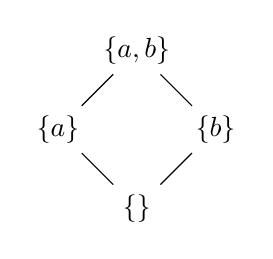
\begin{tikzpicture}
	\node (1) at (0,0) {$\{a,b\}$};
	\node (2) at (-1,-1) {$\{a\}$};
	\node (3) at (1,-1) {$\{b\}$};
	\node (4) at (0,-2) {$\{\}$};
	
	\path [-]
	(1) edge (2)
	(1) edge (3)
	(2) edge (4)
	(3) edge (4);
\end{tikzpicture}\\

\definition{Strong Partial Order}
A \textit{Strong Partial Order} is a relation $\leq$ on a set $S$ that is
\begin{enumerate}[label=\roman*)]
	\item Irreflexive, $\not\exists\ a\in S\ st\ a\leq a$;
	\item Transitive, if $a\leq b\ \&\ b\leq a\implies a=b$; and,
	\item Antisymmetric, if $a\leq b\ \& b\leq c\implies a\leq c\ \forall\ a,b,c\in S$.
\end{enumerate}
\nb This is also known as a \textit{Strict Partial Order}.\\

\example{Strong Partial Order}
Below the \textit{"`put on before`} relation is a \textit{strong partial order}.\\
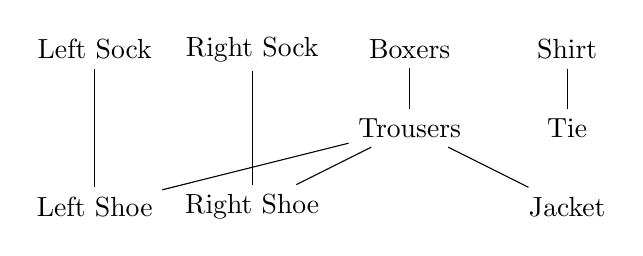
\begin{tikzpicture}
	\node (1) at (0,0) {Left Sock};
	\node (2) at (2,0) {Right Sock};
	\node (3) at (4,0) {Boxers};
	\node (4) at (6,0) {Shirt};
	\node (5) at (4,-1) {Trousers};
	\node (6) at (6,-1) {Tie};
	\node (7) at (0,-2) {Left Shoe};
	\node (8) at (2,-2) {Right Shoe};
	\node (9) at (6,-2) {Jacket};
	
	\path [-]
	(1) edge (7)
	(2) edge (8)
	(3) edge (5)
	(4) edge (6)
	(7) edge (5)
	(8) edge (5)
	(9) edge (5);
\end{tikzpicture}

\definition{Total Partial Order}
A \textit{Total Partial Order} is a relation $\leq$ on a set $S$ that is
\begin{enumerate}[label=\roman*)]
	\item Connex, $a\leq b\ \mathrm{or}\ b\leq a\forall\ a,b\in S$;
	\item Reflexive, $a\leq a\forall\ a\in S$;
	\item Transitive, if $a\leq b\ \& b\leq c\implies a\leq c\ \forall\ a,b,c\in S$; and,
	\item Antisymmetric, if $a\leq b\ \&\ b\leq a\implies a=b$.
\end{enumerate}
\nb This is also known as a \textit{Chain}.\\

\example{Total Partial Order}
Below the $\leq$ relation is a \textit{total partial order}.\\
\begin{tikzpicture}
	\node (1) at (0,0) {$\dots$};
	\node (2) at (1,0) {3};
	\node (3) at (2,0) {2};
	\node (4) at (3,0) {1};
	\node (5) at (4,0) {$\dots$};
	
	\path [-]
	(1) edge (2)
	(2) edge (3)
	(3) edge (4)
	(4) edge (5);
\end{tikzpicture}\\

\definition{Fixpoints}
The \textit{Fixpoints} of a function $f:X\to X$ are all $x$ where $f(x)=x$.\\

\definition{Least Fixpoint}
The \textit{Least Fixpoint} of a function is the lowest \textit{Fixpoint} value.\\

\example{Fixpoints \& Least Fixpoints}
\begin{tabular}{l|l|l}
$f$&fix(f)&lfp(f)\\
\hline
$x\mapsto x^2$&$\{0,1\}$&$0$\\
$x\mapsto 2x$&$\{0\}$&$0$\\
$x\mapsto x+1$&$\{\}$&undefined\\
$x\mapsto x$&$\real$&undefined\\
\end{tabular}

\proposition{Fixpoints Haskell Implementation}
To compute the least fixpoint of a function using Haskell we define the following function
\begin{code}
fix f = f (fix f)
\end{code}

\example{Fixpoints Haskell Implementation}
\begin{code}
fix (*2) = (*2) (fix (*2))
         = (*2) (*2) (fix (*2))
         $\vdots$
         = $\bot$

fix (const 2) = (const 2) (fix (const 2))
              = 2
\end{code}

\remark{Fixpoints in Recursive Functions}
Fixpoints can often be used to redefine recursive functions.\\
This includes factorial
\begin{code}
fac = fix ($\backslash$f n -> if n==0 then 1 else n * f (n-1))
\end{code}

\definition{Trans}
\textit{Trans} is the set of all possible state transformers
$$Trans=(State\hookrightarrow State)$$

\definition{$\sqsubseteq$ Relation}
We define the $\sqsubseteq$ relation over \textit{Trans}
$$\forall\ g_1,g_2\in Trans,\ g_1\sqsubseteq g_2\implies \forall\ s,s'\in State\ \mathrm{if}\ g_1 s=s'\implies g_2 s=s'$$
\nb if $g_1\sqsubseteq g_2$ we say \textit{``$g_1$ shares its results with $g_2$"}.\\

\example{$\sqsubseteq$ Relation}
Consider the following definitions
\[\begin{array}{cc}
g_1\ s=s\ \forall\ s&g_2\ s=\begin{cases}s&\mathrm{if\ }s\ x\geq 0\\ undef& \mathrm{otherwise}\end{cases}\\
g_3\ s=\begin{cases}s&\mathrm{if\ }s\ x= 0\\ undef& \mathrm{otherwise}\end{cases}&g_4\ s=\begin{cases}s&\mathrm{if\ }s\ x\leq 0\\ undef& \mathrm{otherwise}\end{cases}
\end{array}\]
Then $g_3\sqsubseteq g_2\sqsubseteq g_1$ \& $g_3\sqsubseteq g_4\sqsubseteq g_1$ only.\\

\theorem{Type of order, $\sqsubseteq$}
$\sqsubseteq$ is a weak partial order over \textit{Trans}.\\

\proof{Theorem 7.1}
\textit{Reflexivity} - Trivial.\\
\textit{Transitivity}\\
Let $g_1,g_2,g_3$ be arbitrary state transformers with $g_1\sqsubseteq g_2$ \& $g_2\sqsubseteq g_3$.\\
Assume $g_1\ s=s'$ for arbitrary states $s,s'$.\\
$\implies g_2\ s=s'\implies g_3\ s=s'\implies g_1\sqsubseteq g_3$.\\
\textit{Anti-Symmetry}\\
Let $g_1,g_2$ be arbitrary state transformers with $g_1\sqsubseteq g_2$ \& $g_2\sqsubseteq g_1$.\\
Assume $g_1\ s=s'\implies g_2\ s=s'$.\\
If $s'=\bot\implies g_1\ s$ is undefined.\\
if $s'\neq\bot$ then $g_1\ s=s'\implies g_2 s=s'\implies g_1 s=s'\implies g_1=g_2$.\\

\theorem{$\sqsubseteq$ has a least element}
$\sqsubseteq$ has a unique least element.\\
This is the function that is undefined for all states.\\

\definition{Partial Order Set}
Let $\sqsubseteq$ be a partial order on a set $D$.\\
This combination is a \textit{Partial Order Set} (PO-Set).\\
It is denoted $(D,\sqsubseteq)$.\\

\definition{Upper Bound of PO-Set}
Let $Y\subseteq D$ be any subset.\\
The element $d\in D$ is called an \textit{Upper Bound} of $Y$ iff $t\sqsubseteq d\ \forall\ y\in Y$.\\

\definition{Least Upper Bound of Partial Order Set}
Let $Y\subseteq D$ be any subset.\\
The element $d\in D$ is called a least upper bound of $Y$ iff $d\sqsubseteq d'$ forall upper bounds $d'$ of $Y$.\\
\nb We denote $d$ as $\bigsqcup Y$.\\

\remark{Least Upper Bound is Union}
Generally the \textit{Least Upper Bound} of a \textit{Partial Order Set} is the union of all elements of the set.\\

\definition{Chain}
We say that a set $Y\subset D$ is a chain iff $y_1\sqsubseteq y_2$ or $y_2\sqsubseteq y_1\ \forall y_1,y_2\in Y$.\\
This means $Y$ is a totally ordered subset of $D$.\\

\definition{Chain Complete Partial Orders, CCPO}
A \textit{PO-Set} $(D,\sqsubseteq)$ is caled a \textit{Chain-Complete Partially Ordered Set} if the least upper bound $\bigsqcup$ exists for all \underline{chains} $Y\subseteq D$.\\

\definition{Complete Lattice}
A \textit{PO-Set} $(D,\sqsubseteq)$ is caled a \textit{Complete Lattice} if the least upper bound $\bigsqcup$ exists for all \underline{subsets} $Y\subseteq D$.\\

\definition{Monotone Function}
Let $(D,\sqsubseteq)$ and $(D',\sqsubseteq')$ be CCPOs and $f$ be a total function with signature $f:D\to D'$.\\
$f$ is \textit{Monotone} iff $d_1 \sqsubseteq d_2\implies f (d_1)\sqsubseteq' f (d_2)\ \forall\ d_1,d_2\in D$.\\

\definition{Continuous Functions}
Let $(D,\sqsubseteq)$ and $(D',\sqsubseteq')$ be CCPOs and let $f$ be a monotone function with signature $f:D\to D'$.\\
$f$ is \textit{Continuous} iff the following holds $\forall\ Y\subseteq D$ with $Y\neq\emptyset$
$$\bigsqcup\{f d|d\in Y\}=f(\sqcup Y\}$$

\remark{Visual Intuition for Function Analysis}
\includegraphics[scale=0.3]{img/intuitionForFunctions.png}

\theorem{Fixpoint Theorem}
Let $f:D\to D$ be a continuous function on a \textit{Chain Complete Partial Order} $\langle D,\sqsubseteq\rangle$ with least element $\bot$.\\
Then the element $Fix\ f=\bigsqcup\{f^n(\bot)|n\geq0\}\in D$ exists \& is the least fixpoint of $f$.\\
\nb $f^0=id$ \& $f^n=f\cdot f^{n-1}\ \forall n>0$.\\

\proof{Fixpoint Theorem}
First we prove that $Y=\{f^n(\bot)|n\geq0\}$ is a non-empty chain.\\
$\bot\in Y$ trivially, since $f^0(\bot)=\bot$.\\
Since $f^n(\bot)\sqsubseteq f^{n+1}(\bot)\ \forall\ n\geq 0\ \exists\ Fix\ f=\bigsqcup Y$ by the defining property of a chain complete partial order.\\
\\
Next we show that the least upper bound of $Y$ is the least upper bound of $Y$'s image under $f$
\[\begin{array}{rcl}
\bigsqcup Y&=& \bigsqcup\{f^n(\bot)|n\geq0\}\\
&=&\bigsqcup\big\{\{f^n(\bot)|n>0\}\cup\{f^0(\bot)\}\big\}\\
&=&\bigsqcup\big\{\{f^n(\bot)|n>0\}\cup\{bot\}\big\}\\
&=&\bigsqcup\{f^n(\bot)|n>0\}\\
&=&\bigsqcup\{f\cdot f^{n-1}(\bot)|n>0\}\\
&=&\bigsqcup\{f\cdot f^{n'-1}(\bot)|n\geq0\}\\
&=&\bigsqcup\{f(y)|y\in Y0\}
\end{array}\]
Next, we show $Fix\ f$ is a fixpoint of $f$
\[\begin{array}{rcl}
f(Fix\ f)&=&f\left(\bigsqcup Y\right)\\
&=&\bigsqcup\{f(y)|y\in Y\}\\
&=&\bigsqcup Y\\
&=&Fix\ f
\end{array}\]
Finally, we show $Fix\ f$ is the least fixpoint of $f$.\\
Since $f^(\bot)\sqsubseteq f^n(d)\ \forall n>0,\ d\in D$.


\section{Denotational Semantics}

\definition{Denotational Semantics}
A \textit{Denotational Semantics} defines the meaning of a program using a partial function called a \textit{state-transformer} from initial states to final states.\\
\textit{Denotational Semantics} must be compositional (i.e. define expressions in terms of their strict sub-expressions).\\

\remark{Types of Denotational Semantics}
There are two types/flavours of \textit{Denotational Semantics}
\begin{enumerate}[label=\roman*)]
	\item Direct-Style; and,
	\item Continuation-Style.
\end{enumerate} 

\definition{Direct-Style Semantic Function}
A \textit{Direct-Style Semantic Function} has the form
$$\mathcal{S}_{ds}:Stm\to(State\hookrightarrow State)$$

\proposition{Overview of Denotational Semantics}
Here is an overview of how \textit{Denotational Semantics} decomposes common expressions.\\
FIX is the least fixpoint operator \& cond is a conditional function.\\
\begin{tabular}{lcl}
$\mathcal{S}_{ds}$&:&Stm$\to$(State$\hookrightarrow$State)\\
$\mathcal{S}_{ds}[[x:=a]]s$&=&$s[x\mapsto\mathcal{A}[[a]]s]$\\
$\mathcal{S}_{ds}[[skip]]$&=&id\\
$\mathcal{S}_{ds}[[S_1;S_2]]$&=&$\mathcal{S}_{ds}[[S_2]]\cdot\mathcal{S}_{ds}[[S_1]]$\\
$\mathcal{S}_{ds}[[$if $b$ then $S_1$ else $S_2$]]&=&cond($\mathcal{B}[[b]]\mathcal{S}_{ds}[[S_1]],\mathcal{S}_{ds}[[S_2]]$)\\
$\mathcal{S}_{ds}$[[while $b$ do $S$]]&=& FIX $F$ where $F\ g=$cond$(\mathcal{B}[[b]],g\cdot\mathcal{S}_{ds}[[S]],id)$
\end{tabular}
\\

\definition{Conditional Function}
The \textit{Conditional Function} is closely related to the denotational semantics of conditionals \& loops.\\
The \textit{Conditional Function} is defined by\\
\begin{tabular}{rcl}
cond&:&$(X\to T)\times(X\hookrightarrow Y)\times(X\hookrightarrow Y)\to(X\hookrightarrow Y)$\\
cond($b,c,d$)$x$&=&$\begin{cases}c(x)&\mathrm{if\ }b(x)=tt\\d(x)&\mathrm{otherwise}\end{cases}$
\end{tabular}
Where $b$ is our boolean test and $c$ \& $d$ are two functions we want to map with.\\

\proposition{Conditional Function \& Denotational Semantics}
For \textit{Denotational Semantics} we are interested in the case when the \textit{Conditional Function} maps between states
\begin{center}
cond:$(State\to T)\times(State\hookrightarrow State)\times(State\hookrightarrow State)\to(State\hookrightarrow State)$
\end{center}

\definition{Semantics of Assignment}
Here is now \textit{assignment} is defined in denotational semantics\\
\begin{tabular}{lcl}
$\mathcal{S}_{ds}[[x:=a]]s$&=&$s[x\mapsto\mathcal{A}[[a]]s]$\\
$\mathcal{S}_{ds}[[x:=a]]$&=&$\lambda s.s[x\mapsto\mathcal{A}[[a]]s]$\\
$\mathcal{S}_{ds}[[x:=a]]s\ v$&=&$\begin{cases}\mathcal{A}[[a]]s&\mathrm{if\ }v=x\\s\ v&\mathrm{otherwise}\end{cases}$
\end{tabular}
\\
\nb $\lambda$ signifies lambda calculus here.\\

\definition{Semantics of Skip}
Here is now \textit{skip} is defined in denotational semantics\\
\begin{tabular}{lcl}
$\mathcal{S}_{ds}[[$skip$]]$&=&id\\
$\mathcal{S}_{ds}[[$skip$]]$&=&$\lambda s.s$\\
$\mathcal{S}_{ds}[[$skip$]]s$&=&$s$
\end{tabular}
\\
\nb $\lambda$ signifies lambda calculus here.\\

\definition{Semantics of Statement Composition}
Here is now \textit{Statement Composition} is defined in denotational semantics\\
\begin{tabular}{lcl}
$\mathcal{S}_{ds}[[S_1;S_2]]$&=&$\mathcal{S}_{ds}[[S_2]]\cdot\mathcal{S}_{ds}[[S_1]]$\\
$\mathcal{S}_{ds}[[S_1;S_2]]s$&=&$(\mathcal{S}_{ds}[[S_2]]\cdot\mathcal{S}_{ds}[[S_1]])s$\\
&=&$\mathcal{S}_{ds}[[S_2]](\mathcal{S}_{ds}[[S_1]]s)$\\
&=&$s''$ where $s''=\mathcal{S}_{ds}[[S_2]]s'$ and $s'=\mathcal{S}_{ds}[[S_1]]s$
\end{tabular}\\
\nb $\mathcal{S}_{ds}[[S_1;S_2]]s$=undef if $s'=$undef or $s''=$undef.\\

\definition{Semantics of Conditionals}
Here is now \textit{Conditionals} is defined in denotational semantics\\
\begin{tabular}{lcl}
$\mathcal{S}_{ds}[[$if $b$ then $S_1$ else $S_2]]$&=&cond$(\mathcal{B}[[b]],\mathcal{S}_{ds}[[S_1]],\mathcal{S}_{ds}[[S_2]])$\\
$\mathcal{S}_{ds}[[$if $b$ then $S_1$ else $S_2]]s$&=&cond$(\mathcal{B}[[b]],\mathcal{S}_{ds}[[S_1]],\mathcal{S}_{ds}[[S_2]])s$\\
&=&$\begin{cases}\mathcal{S}_{ds}[[S_1]]s&\mathrm{if\ }\mathcal{B}[[b]]s=tt\\\mathcal{S}_{ds}[[S_2]]s&\mathrm{otherwise}\end{cases}$
\end{tabular}\\
\nb $\mathcal{S}_{ds}[[$if $b$ then $S_1$ else $S_2$ $]]s$=undef if the statement it calls is undefined in states $s$.\\

\definition{Semantics of Loops}
Here is now \textit{Loops} is defined in denotational semantics\\
\begin{tabular}{lcl}
$\mathcal{S}_{ds}[[$while $b$ do $S]]$&=&FIX $F$ where $F\ g=$ cond($\mathcal{B}[[b]],g\cdot\mathcal{S}_{ds}[[S]],id)$
Since\\
$\mathcal{S}_{ds}[[$while $b$ do $S]]$&=&$\mathcal{S}_{ds}[[$if $b$ then $(S;$ while $b$ do $S)$ else skip$]]$\\
&=&cond($\mathcal{B}[[b],\mathcal{S}_{ds}[[S;$ while $b$ do $S]],\mathcal{S}_{ds}[[$skip$]])$\\
&=&cond($\mathcal{B}[[b],\mathcal{S}_{ds}[[$ while $b$ do $S]]\cdot\mathcal{S}_{ds}[[S]])$\\
&$\in$&$fix(\lambda g$.cond($\mathcal{B}[[b]],g\cdot\mathcal{S}_{ds}[[S]],id))$\\
&=&FIX $(\lambda g$.cond($\mathcal{B}[[b]],g\cdot\mathcal{S}_{ds}[[S]],id))$\\
\end{tabular}\\
\nb $\mathcal{S}_{ds}[[$while $b$ do $S]]s$=undef if $($FIX$\ F)s$=undef.\\
\nb $\lambda$ signifies lambda calculus here.\\

\definition{Functional of a Loop}
The \textit{Functional of the Loop} while $b$ do $s$, when it is defined as
$$F:=\lambda g.\mathrm{cond}(\mathcal{B}[[b]],g\cdot\mathcal{S}_{ds}[[S]],id$$
The functional can be seen as a means of finding better approximations to the semantics of the loop as it can be shown that \begin{center}
$F^n(\emptyset)$ is a correct semantics for all states from which the loop ends in fewer than $n$ iterations.
\end{center}
\nb $\lambda$ signifies lambda calculus here.\\

\proposition{Characterisation of the Functional of a Loop}
A \textit{direct characterisation} of $F$ is any equivalent mathematical expression that does not contain any semantic functions.\\

\remark{Definition of Loop is insufficient}
The fixpoint functional definition for the semantics of loops is not sufficient
\begin{center}
$\mathcal{S}_{ds}[[$while $b$ do $S]]$=FIX $F$ where $F\ g=$ cond($\mathcal{B}[[b]],g\cdot\mathcal{S}_{ds}[[S]],id)$
\end{center}
It faces two problems
\begin{enumerate}[label=\roman*)]
	\item There are functional that have more than one fixed point;
	\item There are functionals that have no fixed points.\\
\end{enumerate}

\proposition{Defining Semantics for Loops using Fixpoints}
The following example shows that fixpoints of a loop functional are not sufficient, in themselves, to provide a semantics for loops as more than one such fixpoint may exist.\\
Consider the loop {\ttfamily{while $\neg(x=0)$ do skip}}. The function $F$ of this is defined as
\begin{center}
{\ttfamily{F g=cond($\mathcal{B}[[\neg(x=0)]],\ g\cdot\mathcal{S}_{ds}[[skip]]$, id)}}
\end{center}
Thus {\ttfamily F g s =}$\begin{cases}g\ s&\mathrm{if\ }s\ x\neq0\\s&\mathrm{if\ }s\ x=0\end{cases}$
.\\
From this we can identify the fixpoints $s$ where
\begin{center}
{\ttfamily{g s = F g s =}}$\begin{cases}g\ s&\mathrm{if\ }s\ x\neq0\\s&\mathrm{if\ }s\ x=0\end{cases}$
\end{center}
But since $g\ s==g\ s$ is always true the top condition is redundant and so a fixpoint of $F$ is just any function $g$ st $g\ s=s$ \textit{i.e.} where $s\ x=0$.\\
Thus the least fixpoint is undefined whenever $s\ x\neq 0$, even though other fixpoints exists (e.g. id).\\

\remark{Functionals with no fixpoints}
Let $g_1$ \& $g_2$ be any state transformers st $g1\neq g2$.\\
Define the functional $F$ as
$$F\ g=\begin{cases}g_1&\mathrm{if\ }g=g_2\\g_2&\mathrm{otherwise}\end{cases}$$

\remark{Motivation to Solution to Remark 7.3}
Consider the three possible outcomes for a state $s_0$ in a loop
\begin{enumerate}[label=\roman*)]
	\item Loop Terminates\\
	\textit{e.g.} The loop {\ttfamily{while $0\leq x$ do $x:=x-1$}} terminates $\forall\ s_0$ where $x\geq0$.
	\item Loops Locally, loops due to a construct with statement $S$.\\
	\textit{e.g.} The loop {\ttfamily{while $0\leq x$ do (if $x=0$ then (while true do skip) else $x:=x-1$}} ends up looping once $x=0$ $\forall\ s_0$ where $x\geq0$.
	\item Loops Globally, loops due to condition $b$.\\
	\textit{e.g.} The loop {\ttfamily{while $\neg(x=0)$ do skip}} loops $\forall\ s_0$ where $x\neq0$.\\
\end{enumerate}

\section{Static Program Analysis}
THIS CHAPTER IS NON-EXAMINABLE.

\section{Axiomatic Semantics}

\remark{Motivation}
Generally we are more interested in some properties of a program, than others.\\
The more interesting properties tend to be those related to the intended purpose of the program, rather than incidental results due to a particular implementation.\\
\textit{e.g.} Given {\ttfamily{while $\neg$(x=1) do (u:=y*x; x:=x-1)}} we are interested that $y=n!$ when initially $y=1$ \& $n>0$, but not interested in the final value of $x$.\\

\definition{Partial Correctness Properties}
\textit{Partial Correctness Properties} state that \underline{if} a program terminates then a certain relationship will hold between the initial \& final variable values.\\

\definition{Total Correctness Properties}
\textit{Total Correctness Properties} state that a program \underline{will} terminate and a certain relationship will hold between the initial and final variables values.\\

\remark{Axiomatic Semantics \& Correctness Properties}
An \textit{Axiomatic Semantics} allows us to prove a program satisfies formal partial or total correctness properties.\\

\definition{Axiomatic Semantics}
An \textit{Axiomatic Semantics} consists of a set of axioms/rules that provide a method for finding true assertions.\\
An \textit{Axiomatic Semantics} formalises interesting properties of a program by defining pre-conditions \& post-conditions.\\

\remark{Transitions of Axiomatic Semantics}
An \textit{Axiomatic Semantics} will have a single assertion $a$, the conclusion, and one or more assertions $a_1,\dots,a_n$, premises, which are required to prove $a$ holds
$$\dfrac{a_1\dots a_n}{a}$$

\definition{Hoare Triples}
\textit{Hoare Triples} are the standard way of denoting axiomatic semantics
\begin{center}
Pre-Condition Program Post-Condition
\end{center}
\nb The conditions are known as assertions.\\

\remark{Partial Correctness Semantics \& Hoare Triples}
Under the \textit{Partial Correctness Semantics} assertions are written as $\{P\}\ S\ \{R\}$.\\
This means that if $P$ holds before running $S$ \underline{and} $S$ terminates, then $R$ will hold immediately after.\\

\remark{Total Correctness Semantics \& Hoare Triples}
Under the \textit{Total Correctness Semantics} assertions are written as $\{P\}\ S\ \{\Downarrow R\}$ or $[P]\ S\ [R]$.\\
This means that if $P$ holds before running $S$ then $R$ will hold immediately after.\\

\definition{Logical Variables}
\textit{Logical Variables} are variables that are not defined in the running of a program, but can be derived from program variables.\\
\nb Commonly \textit{Logical Variables} are used to remember past values of program variables.\\

\definition{Schemata}
\textit{Schemata} are used to define individual axioms \& contain meta-variables that may be instantiated for particular pre \& post-conditions.\\

\proposition{Intentional Partial Correctness Schemata}
\[\begin{array}{ll}
\{P\}\ skip\ \{P\}&\mathrm{Skip}\\
\{P(a)\}\ x:=a\ \{P(x)\}&\mathrm{Assertion}\\
\dfrac{\{P\}\ S_1\ \{R\}\quad\{R\}\ S_2\ \{Q\}}{\{P\}S_1;S_2\{Q\}}&\mathrm{Composition}\\
\dfrac{\{P\wedge b\}\ S_1\ \{Q\}\quad\{P\wedge\neg b\}\ S_2\ \{Q\}}{\{P\}if\ b\ then\ S_1\ else\  S_2\{Q\}}&\mathrm{Conditional}\\
\dfrac{\{P\wedge b\}\ S\ \{P\}}{\{P\}\ while\ b\ do\ S\{P\wedge\neg b\}}&\mathrm{Loop}\\
\dfrac{\{P'\}\ S\ \{Q'\}}{\{P\}\ S\ \{Q\}}\mathrm{if}\ P\vDash P'\ \& Q'\vDash Q P&\mathrm{Consequence}\\
\end{array}\]
\nb $P\vDash Q\implies$ if $P$ is true then $Q$ is true.\\

\proposition{Extensional Partial Correctness Schemata}
\[\begin{array}{ll}
\{P\}\ skip\ \{P\}&\mathrm{Skip}\\
\{P[x\mapsto A_{[[a]]}]\}\ x:=a\ \{P\}&\mathrm{Assertion}\\
\dfrac{\{P\}\ S_1\ \{R\}\quad\{R\}\ S_2\ \{Q\}}{\{P\}\ S_1; S_2\ \{Q\}}&\mathrm{Composition}\\
\dfrac{\{P\wedge B+{[[b]]}\}\ S_1\ \{Q\}\quad\{P\wedge\neg B_{[[b]]}\}\ S_2\ \{Q\}}{\{P\}\ if\ b\ then\ S_1\ else\ S_2\ \{Q\}}&\mathrm{Conditional}\\
\dfrac{\{P\wedge B_{[[b]]}\}\ S\ \{P\}}{\{P\}\ while\ b\ do\ S \{P\wedge\neg B_{[[b]]}\}}&\mathrm{Loop}\\
\dfrac{\{P'\}\ S\ \{Q'\}}{\{P\}\ S\ \{Q\}}\ \mathrm{if}\ P\implies P'\ \&\ Q'\implies Q&\mathrm{Consequence}\\
\end{array}\]

\remark{Using Consequence Rule}
One should avoid using the \textit{Consequence Rule} unless no other rules would be valid.\\
When used you need to also prove that the new conditions ($P'$ \& $Q'$) do satisfy $P\vDash P'$ \& $Q'\vDash Q$.\\

\example{Modulus}
\[
\dfrac
{\dfrac{\{(x-2)\%2=n\%2\ \&\&\ x-2\geq0\}\ x:=x-2\ \{x\%2=n\%2\ \&\&\ x\geq0\}}
{\dfrac
{\{x\%2=n\%2\ \&\&\ x\geq0\ \&\&\ 2\leq x\}\ while\ 2\leq x\ do\ x:=x-2\ \{x\%2=n\%2\\ \&\&\ x\geq0\}}
{\{x\%2=n\%2\ \&\&\ x\geq0\}\ while\ 2\leq x\ do\ x:=x-2\ \{x\%2=n\%2\\ \&\&\ x\geq0\ \&\&\ \neg(2\leq x)\}}
}}
{\{x=n\ \&\&\ n\geq0\}\ while\ 2\leq x\ do\ x:=x-2\ \{x=n\%2\}}
\]

\proposition{Total Correctness Schemata}
\[\begin{array}{ll}
[P]\ skip\ [P]&\mathrm{Skip}\\
\left[P(a)\right]\ x:=a \left[P(x)\right]&\mathrm{Assignment}\\
\dfrac{\left[P\right]\ S_1\ \left[Q\right]\quad\left[Q\right]\ S_2\ \left[R\right]}{\left[P\right]\ S_1;S_2\ \left[R\right]}&\mathrm{Composition}\\
\dfrac{\left[P\wedge b\right]\ S_1\ \left[Q\right]\quad\left[P\wedge\neg b\right]\ S_2\ \left[Q\right]}{\left[P\right]\ if\ b\ then\ S_1\ else\ S_2\ \left[Q\right]}&\mathrm{Conditional}\\
\dfrac{\left[P(z+1)\right]\ S\ \left[P(z)\right]}{\left[\exists\ z\in\nats\ P(z)\right]\ while\ b\ do\ S\ \left[P(0)\right]}\ if\ \begin{array}{l}
\vDash\ \forall\ z\in\nats\ P(z+1)\implies b\\
\vDash\ P(0)\implies\neg b
\end{array}&\mathrm{Loop}\\
\dfrac{\left[P'\right]\ S\ \left[Q'\right]}{\left[P\right]\ S\ \left[Q\right]}\ if\ \begin{array}{l}\
P\vDash P'\\
Q'\vDash Q
\end{array}&\mathrm{Consequence}\\
\end{array}\]

\newpage
\setcounter{section}{-1}
\section{Reference}
\subsection{The While Language}

\definition{While}
\textit{While} is a simple Turing-Complete language which has the following \textit{syntactic categories}\\
\begin{tabular}{rl}
Numerals&0,1,2,$\dots$\\
Variables&x,y,temp,$\dots$\\
Arithmetics&+,*,-\\
Booleans& true,false,=,$\leq$,$\neg$,$\wedge$\\
Statements& :=, ;, skip, if$\dots$then$\dots$else, while$\dots$do
\end{tabular}
\\

\definition{Meta-Variables}
\textit{Meta-Variables} are the notation used to denote the category of a generic variable.\\
Subscripts \& priming notation is used to distinguish between variables of the same category.\\
The following are the \textit{meta-variables} for each category\\
\begin{tabular}{rl}
Num&$n$\\
Var&$x$\\
Aexp&$a$\\
Bexp&$b$\\
Statement&$S$
\end{tabular}
\\

\definition{Basis Element}
A \textit{boolean expression} is said to be a basis element if it is {\ttfamily{true}}, {\ttfamily{false}} or has the form $a_1=a_2$ or $a_1\leq a_2$.\\
\nb Either is is a standard value or compares arithmetic expressions.\\

\definition{Composite Element}
A \textit{boolean expression} is said to be a \textit{Composite Element} if it has the form $b_1\wedge b_2$ or $\neg b$.\\
\nb It compares boolean expressions.\\

\definition{Abstract Syntax of While}
There are three types of abstract syntax in the \textit{While} language: Arithmetic Expressions, Boolean Expressions; \& Statements\\
\begin{tabular}{rcl}
Aexp&::=&Num|Var\\
&\textbar&Aexp `+' Aexp\\
&\textbar&Aexp `*' Aexp\\
&\textbar&Aexp `-' Aexp\\
Bexp&::=&`true'\textbar`false'\\
&\textbar&Aexp `=' Aexp\\
&\textbar&Aexp `$\leq$' Aexp\\
&\textbar&`$\neg$' Bexp\\
&\textbar&Bexp `$\wedge$' Bexp\\
Stm&::=&Var`:='Aexp\\
&\textbar&`skip'\\
&\textbar&Stm`;'StmAexp\\
&\textbar&`if' Bexp `then' Stm `else; Stm\\
&\textbar&`while' Bexp `do' Stm\
\end{tabular}

\definition{Concrete Syntax of While}
The follow are concrete syntaxes of \textit{While}\\
\begin{tabular}{rcl}
Digit&::=& `0'\textbar`1'\textbar$\dots$\textbar`9'\\
Letter&::=& `a'\textbar`b'\textbar$\dots$\textbar`z'\\
String&::=&$\epsilon$\textbar Digit String \textbar Letter String\\
Num&::=&Digit\textbar Digit Num\\
Var&::=& Letter String\\
Id&::=& Num\textbar Var\\
Factor&::=&Id\textbar Factor `*' Id\\
Aexp&::=& Factor \textbar Aexp `+' Factor \textbar Aexp `-' Factor\\
Atom&::=& `true'\textbar `false'\textbar Aexp `=' Aexp\textbar Aexp `$\leq$' Aexp\\
Literal&::=& Atom\textbar `$\neg$' Literal\\
Bexp&::=& Literal\textbar Bexp`$\wedge$'Literal
\end{tabular}
\\

\proposition{Update Notation}
$f[x\mapsto y]$ is a function that updates the function $f$ to return $y$ for value $x$
$$(f[x\mapsto y])x'=\begin{cases}y&\mathrm{if\ }x'=x\\ f\ x'&\mathrm{otherwise}\end{cases}$$

\definition{Arithmetic Semantics}
Here is a definition for the function $\mathcal{A}$ which returns the value of arithmetic expressions\\
\begin{tabular}{rcl}
$\mathcal{A}$&:&Aexp$\to$(State$\to\mathbb{Z}$)\\
$\mathcal{A}[[n]]$s&=&$\mathcal{N}[[n]]$\\
$\mathcal{A}[[x]]$s&=&sx\\
$\mathcal{A}[[a_1+a_2]]$s&=&$\mathcal{A}[[a_1]]$s+$\mathcal{A}[[a_2]]$s\\
$\mathcal{A}[[a_1*a_2]]$s&=&$\mathcal{A}[[a_1]]$s*$\mathcal{A}[[a_2]]$s\\
$\mathcal{A}[[a_1-a_2]]$s&=&$\mathcal{A}[[a_1]]$s-$\mathcal{A}[[a_2]]$s
\end{tabular}
\\

\definition{Boolean Semantics}
Here is a definition for the function $\mathcal{B}$ which returns the boolean value of an expression.\\
\begin{tabular}{rcl}
$\mathcal{B}$&:&Bexp$\to$(State$\to$Atom)\\
$\mathcal{B}[[\mathrm{true}]]$&=&tt\\
$\mathcal{B}[[\mathrm{false}]]$&=&ff\\
$\mathcal{B}[[a_1=a_2]]$&=&$\begin{cases}\mathrm{tt}&\mathrm{if\ }\mathcal{A}[[a_1]]s=\mathcal{A}[[a_2]]s\\\mathrm{ff}&\mathrm{if\ }\mathcal{A}[[a_1]]s\neq\mathcal{A}[[a_2]]s\end{cases}$\\
$\mathcal{B}[[a_1\leq a_2]]$&=&$\begin{cases}\mathrm{tt}&\mathrm{if\ }\mathcal{A}[[a_1]]s\leq\mathcal{A}[[a_2]]s\\\mathrm{ff}&\mathrm{if\ }\mathcal{A}[[a_1]]s>\mathcal{A}[[a_2]]s\end{cases}$\\
$\mathcal{B}[[\neg b]]$&=&$\begin{cases}\mathrm{tt}&\mathrm{if\ }\mathcal{B}[[b]]s=\mathrm{ff}\\\mathrm{ff}&\mathrm{if\ }\mathcal{B}[[b]]s=\mathrm{tt}\end{cases}$\\
$\mathcal{B}[[a_1\wedge a_2]]$&=&$\begin{cases}\mathrm{tt}&\mathrm{if\ }\mathcal{B}[[b_1]]s=\mathrm{tt\ and\ }\mathcal{B}[[b_2]]s=\mathrm{tt}\\\mathrm{tt}&\mathrm{if\ }\mathcal{B}[[b_1]]s=\mathrm{ff\ or\ }\mathcal{B}[[b_2]]s=\mathrm{ff}\end{cases}$\\
\end{tabular}
\\

\definition{Binary Number Semantics}
Here is a definition for the function $\mathcal{N}$ which returns the denary value of binary number\\
\begin{tabular}{rcl}
$\mathcal{N}$&:&Num$\to\mathbb{Z}$\\
$\mathcal{N}[[0]]$&=&0\\
$\mathcal{N}[[1]]$&=&1\\
$\mathcal{N}[[n\ 0]]$&=&2*$\mathcal{N}[[n]]$\\
$\mathcal{N}[[n\ 1]]$&=&1+2*$\mathcal{N}[[n]]$
\end{tabular}

\end{document}